\chapter{\label{ch:4-accel}Dependence Graph Model for FMU Co-simulation}

\minitoc

This chapter describes a dependence graph model that we propose for representing an FMU co-simulation. The different phases for building such model are explained including the initial construction of the dependence graph, transformations that it undergoes in order to represent multi-rate co-simulation and mutual exclusion constraints, and finally rules for characterizing the graph with real-time parameters.
 
\section{\label{sec:4-depgrph}Dependence Graph of an FMU Co-simulation}

Automatic parallelization of computer programs embodies the adaptation of the potential parallelism inherent in the program to the effective parallelism that is provided by the hardware. Because computer programs are usually complex (multiple functions, nested function calls, control flow jumps, etc.), this process of adaptation requires the use of a model for abstracting the program to be parallelized. The aim of using such model is to identify which parts of the program can be executed in parallel by expressing some features of the program such as data dependence between different parts. Dependence graphs are commonly used for this purpose (see Section \ref{subsec:parsched}). A dependence graph, denoted $G(V,A)$, where $V$ is the set of vertices and $A$ is the set if arcs, defines the partial order to be respected when executing a set of tasks. This partial order describes the potential parallelism of the program, i.e. vertices that are not in precedence relation $A$ which is asymmetric and transitive. %Figure \ref{} shows an example of a task dependence graph of size $5$.

The co-simulation of FMUs lends itself to the dependence graph representation as shown hereafter. According to the FMI standard, the code of an FMU can be exported in the form of source code or as precompiled binaries. However, most FMU providers tend to adopt the latter option for proprietary reasons. We are, thus, interested in this case. The method for automatic parallelization of FMU co-simulation that we propose in this thesis is based on representing the co-simulation by a dependence graph. We present in the rest of this section how this graph is constructed and a set of attributes that characterize it. The graph construction and characterization method is part of the RCOSIM approach as presented in \cite{benkhaled:2014}.

\subsection{Construction of the Dependence Graph of an FMU Co-Simulation}

The entry point for the construction of a dependence graph of an FMU co-simulation is a user-specified set of interconnected FMUs as depicted in Figure~\ref{fig:2mdlsbb}. At this stage, we consider only co-simulations where all FMUs are assigned identical communication step sizes (this restriction is relaxed in Section \ref{sec:opgraph}). We refer to the graph which represents such co-simulation as \textit{mono-rate} graph. The execution of each FMU is seen as computing a set of inputs, a set of outputs, and the state of the FMU. A computation of an input, output, or the state is performed by FMU C function calls. An input (resp. output ) is computed by calling the \textit{fmiSet} (resp. \textit{fmiGet}) function and the state is computed by calling \textit{SetTime, GetDerivatives, SetContinuousStates, etc.}, functions in the case of FMI for Model Exchange or the \textit{DoStep} function in the case of FMI for Co-Simulation. Thanks to FMI, it is additionally possible to access information about the internal structure of a model encapsulated in an FMU. In particular, as shown in Figure~\ref{fig:2mdlsintra}, FMI allows the identification of Direct Feedthrough (e.g. $Y_{B1}$) and Non Direct Feedthrough (e.g. $Y_{A1}$) outputs of an FMU and other information depending on the version of the standard:

\begin{itemize}
\item FMI 1.0: Dependence between inputs and outputs is given. The computation of the state at a given time step $t_k$ is considered necessary for the computation of every output at the same time step $t_k$. It is considered that the computation of the state at a simulation step $t_{k+1}$ requires the computation of each of the inputs at the simulation step $t_{k}$.
\item FMI 2.0: In addition to the information provided in FMI 1.0, more information is given about data dependence. It is specified which output at a given time step depends on the state computation at the same step. Also, it is specified which input at time step $t_k$ needs to be computed before the computation of the state at the step $t_{k+1}$.  
\end{itemize}

\begin{figure}[htb]
\centering
\begin{subfigure}{.5\textwidth}
  \centering
  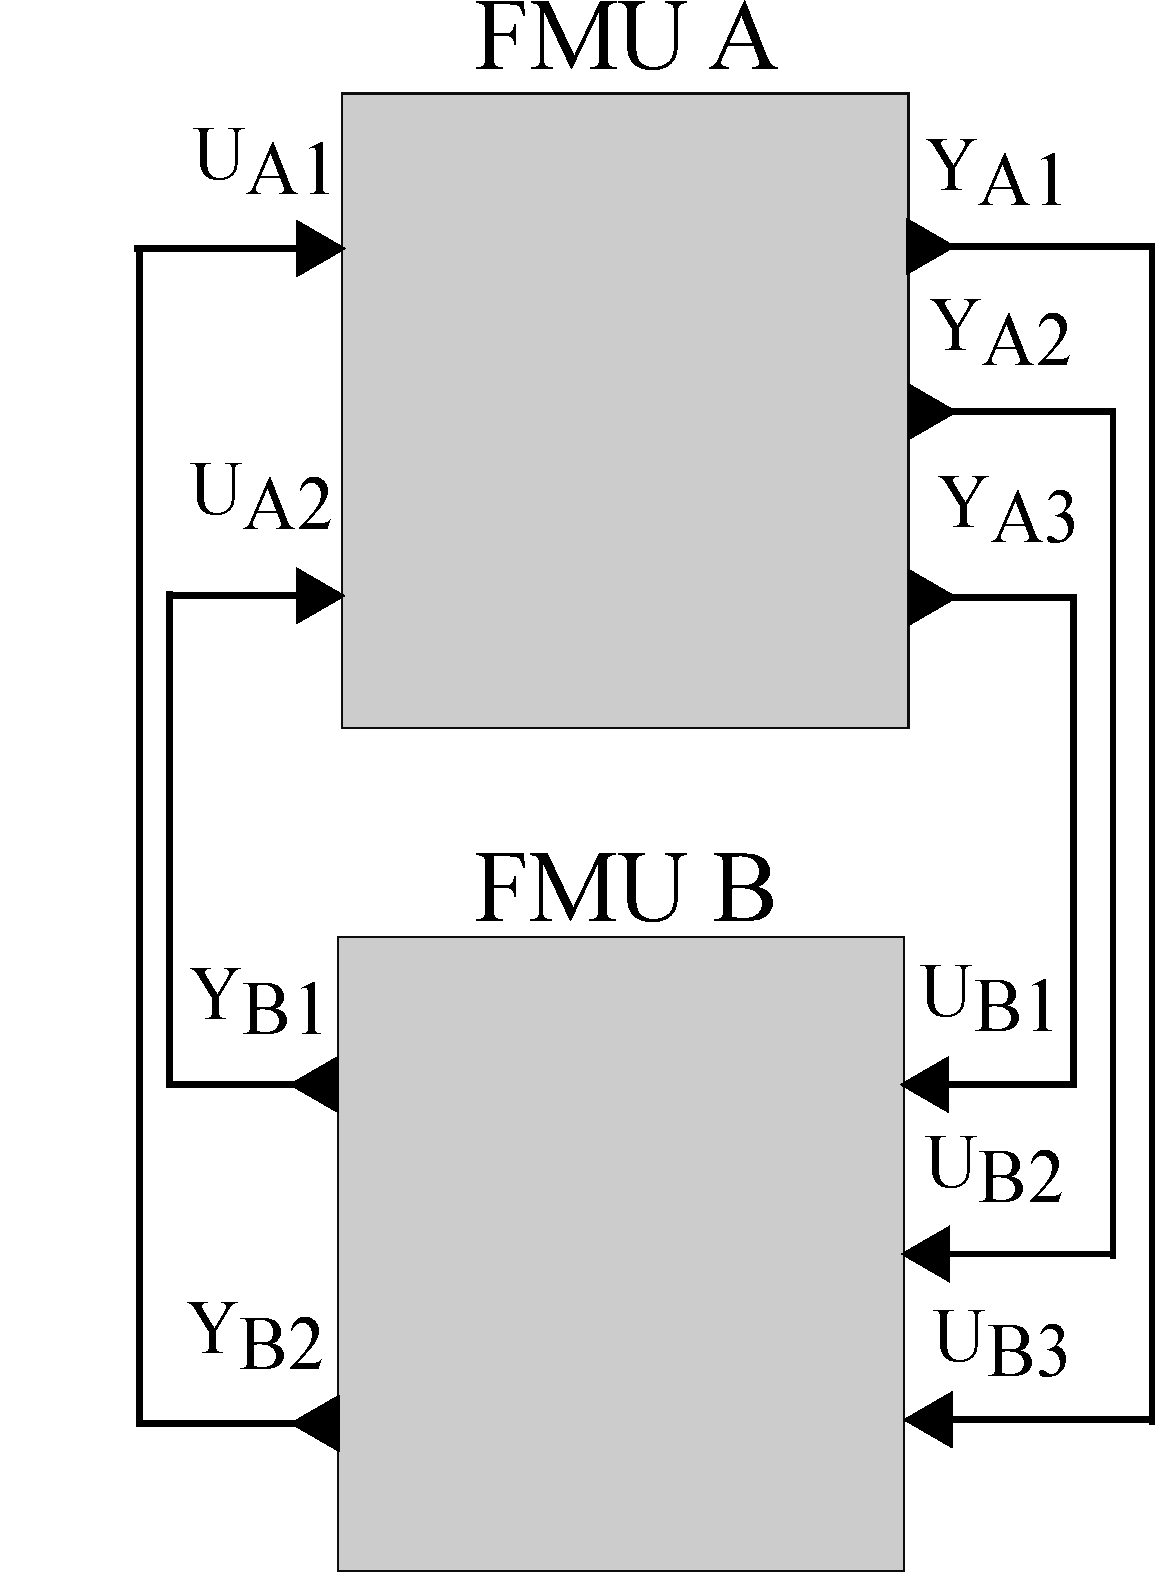
\includegraphics[scale=0.2]{figures/Two_Models_Black_Box}
  \caption{Inter-FMU dependence specified by the user}
  \label{fig:2mdlsbb}
\end{subfigure}%
\begin{subfigure}{.5\textwidth}
  \centering
  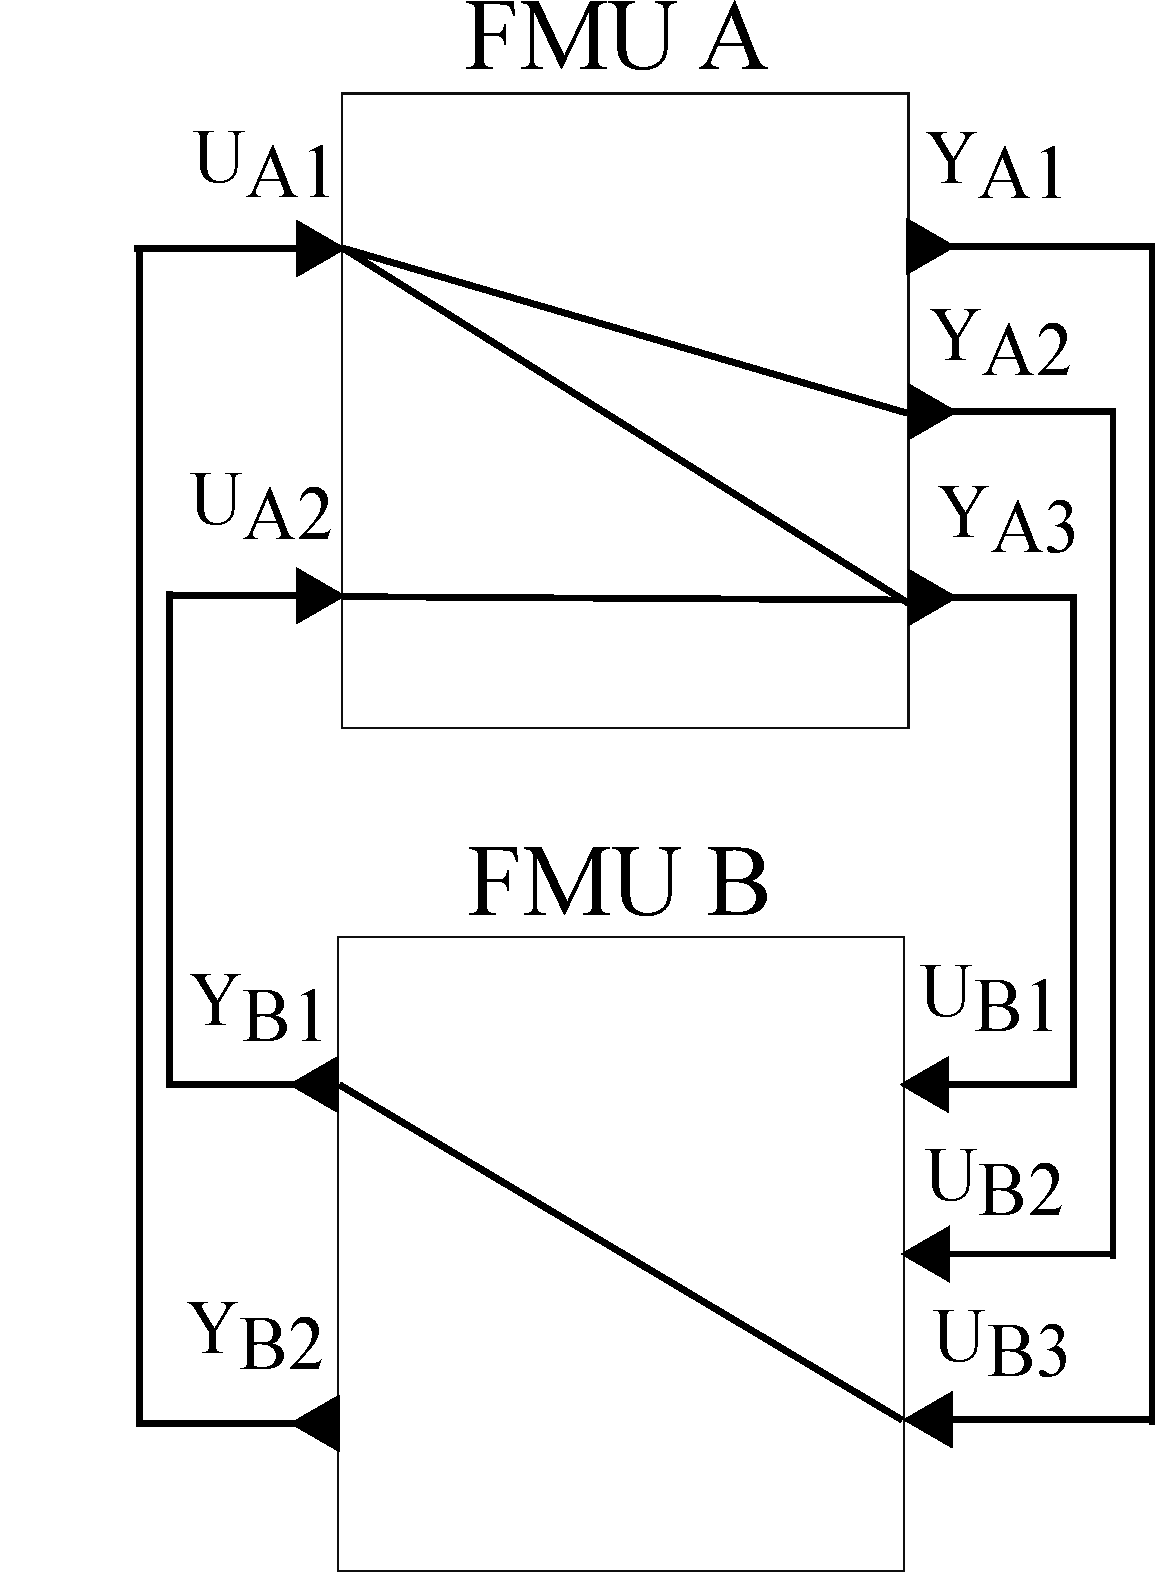
\includegraphics[scale=0.2]{figures/Two_Models}
  \caption{Intra-FMU dependence provided by FMI}
  \label{fig:2mdlsintra}
\end{subfigure}
\caption{An example of inter and intra-FMU dependence of two FMUs connected by the user}
\label{fig:2mdls}
\end{figure}

The information provided by FMI on input-output dependence allows transforming the FMU graph into a graph with an increased granularity. For each FMU, the inputs, outputs, and state are transformed into operations. An input, output, or state operation is defined as the set of FMU function calls that are used to compute the corresponding input, output, or state respectively. The co-simulation is described by a dependence graph $G(V,A)$, called the operation graph, where each vertex $o_i \in V: 0 \leq i < n$ represents one operation, each arc $(o_i,o_j) \in A: 0 \leq i,j < n$ represents a precedence relation between operations $o_i$ and $o_j$, and $n = |V|$ is the size of the operation graph. The operation graph is built by exploring the relations between the FMUs and between the operations of the same FMU. A vertex is created for each operation and arcs are then added between vertices if a precedence dependence exists between the corresponding operations. If FMI 1.0, which does not give information about the dependence between the state computation and the input and output variables computations, is used, we must add arcs between all input operations and the state operation of the same FMU. Furthermore, arcs connect all output operations and the state operation of the same FMU because the computation at the time step $t_k$ of an output must be performed with the same value of the state (computed at simulation step $t_k$) as for all the outputs belonging to the same FMU. An execution of the obtained graph corresponds to one simulation step. Therefore, running the co-simulation consists in repeatedly executing the graph until the desired number of steps is reached. A new execution of the graph cannot be started unless the previous one was totally finished. The operation graph corresponding to the FMUs of Figure~\ref{fig:2mdls} is shown in Figure~\ref{fig:dag}.

\begin{figure}[htb]
\centering
  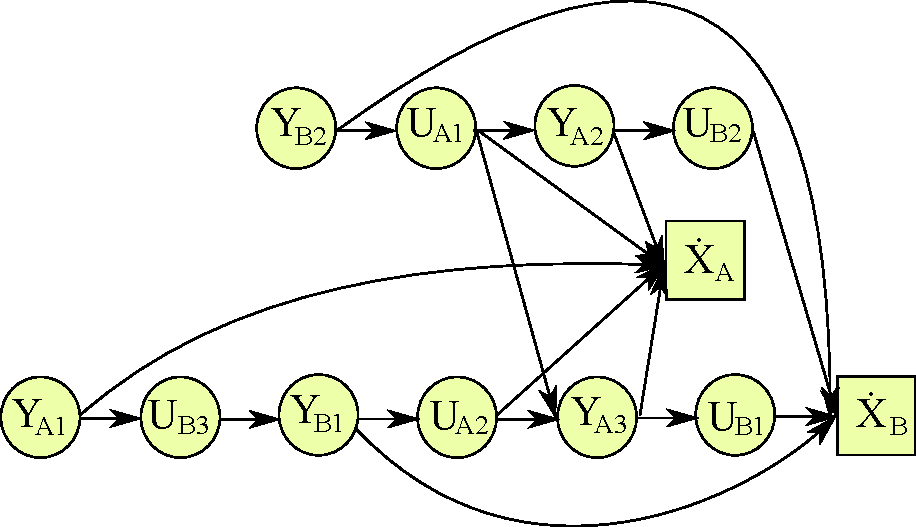
\includegraphics[scale=0.5]{figures/Operation_Graph_Two_Models}
\caption{Operation graph obtained from the FMUs of Figure~\ref{fig:2mdls}}
\label{fig:dag}
\end{figure} 

\subsection{Dependence Graph Attributes}

%In the remainder of the thesis, we shall use the term operation graph instead of operation dependence graph. 
The operation graph is used as input to a scheduling algorithm. In addition to the partial order defined by the graph, the scheduling algorithm uses a number of attributes to compute an efficient schedule of the operation graph. Many list scheduling algorithms use attributes that are computed by the Critical Path Method \cite{kohler:1975}. Below, we define a set of attributes and notations to characterize the operation graph.

The notation $tpe(o_i)$ is used to refer the type of the operation $o_i$, i.e. $tpe(o_i) \in \{update_{input}, update_{output}, update_{state}\}$, and $f_m(o_i)$ denotes the FMU to which the operation $o_i$ belongs. Operation $o_j$ is a predecessor of operation $o_i$ if there is an arc from $o_j$ to $o_i$, i.e. $(o_j, o_i) \in A$. We denote the set of predecessors of $o_i$ by $pred(o_i)$. Operation $o_j$ is an ancestor of operation $o_i$ if there is a path in $G$ from $o_j$ to $o_i$. The set of ancestors of $o_i$ is denoted by $ance(o_i)$. Operation $o_j$ is a successor of operation $o_i$ if there is an arc from $o_i$ to $o_j$, i.e. $(o_i, o_j) \in A$. We denote the set of successors of $o_i$ by $succ(o_i)$. Operation $o_j$ is a descendant of operation $o_i$ if there is a path in $G$ from $o_i$ to $o_j$. The set of descendants of $o_i$ is denoted by $desc(o_i)$. A profiling phase allows measuring the execution time of each operation $o_i \in V$, denoted $C(o_i)$. For each operation, the average execution time of multiple co-simulation runs is used. When co-simulation under real-time constraints is aimed, Worst Case Execution Times (WCET) are used instead. An operation $o_i$ is characterized by its communication step $H(o_i)$ which is equal to the communication step assigned to the FMU $f_m(o_i)$. The earliest start time from start denoted $S(o_i)$ and the earliest end time form start denoted $E(o_i)$ are defined by equations \ref{eq:sfs} and \ref{eq:efs} respectively. $S(o_i)$ is the earliest time at which the operation $o_i$ can start its execution. $S(o_i)$ is subject to constraints imposed by precedence relations. The earliest time the operation $o_i$ can finish its execution is $E(o_i)$.

\begin{equation}
S(o_i)=\begin{cases}
    0, & \text{if $pred(o_i)=\emptyset$}.\\
    max_{o_j \in pred(o_i)}(E(o_j)), & \text{otherwise}.
  \end{cases}
	\label{eq:sfs}
\end{equation}

\begin{equation}
	E(o_i)=S(o_i)+C(o_i) 
	\label{eq:efs}
\end{equation}

The latest end time from end denoted $\overline{E}(o_i)$ and the latest start time from end denoted $\overline{S}(o_i)$ are defined by equations \ref{eq:efe} and \ref{eq:sfe} respectively. %$\overline{E}(o_i)$ defines the latest time by which the operation $o_i$ must finish its execution so as not to increase the total execution time of the graph. For $o_i$ to finish its execution no later than $\overline{E}(o_i)$, it has to start its execution at the latest at $\overline{S}(o_i)$. 

\begin{equation}
\overline{E}(o_i)=\begin{cases}
    0, & \text{if $succ(o_i)=\emptyset$}.\\
    max_{o_j \in succ(o_i)}(\overline{S}(o_j)), & \text{otherwise}.
  \end{cases}
	\label{eq:efe}
\end{equation}

\begin{equation}
	\overline{S}(o_i)=\overline{E}(o_i)+C(o_i) 
	\label{eq:sfe}
\end{equation}

The critical path of the graph is the longest path in the graph. The length of a path is computed by accumulating the execution times of the operations that belong to it. The length of the critical path of the operation graph denoted by $R$ is defined by equation \ref{eq:crit}. The critical path is a very important characteristic of the operation graph. It defines a lower bound on the execution time of the graph, i.e. in the best case, the time needed to execute the whole graph is equal to the length of the critical path. 

\begin{equation}
	R = \max_{o_i \in V}(E(o_i)) 
	\label{eq:crit}
\end{equation}
 
The flexibility $F(o_i)$ is defined by equation \ref{eq:flex}. It expresses the length of a time interval within which operation $o_i$ can be executed without increasing the total execution time of the graph.

\begin{equation}
	F(o_i) = R - S(o_i) - C(o_i) - \overline{E}(o_i) 
	\label{eq:flex}
\end{equation}

\section{\label{sec:opgraph}Dependence Graph of a Multi-rate FMU Co-simulation}

The operation graph model presented in the previous section allows modeling only mono-rate FMU co-simulations. For some applications this model is sufficient to be used for multi-core scheduling. However, many industrial co-simulation applications feature behaviors that cannot be captured by this model. In particular, many industrial applications involve FMUs that are executed according to different communication step sizes. This is especially true when different FMUs of a co-simulation are provided by different parties. It is very common that an FMU provider designs the FMU in such a way that its proper functioning depends on using specific communication step sizes. It is, therefore, highly unrecommended, and in some cases even impossible, to change the communication step size of the FMU. In other cases, even if it is possible and acceptable to change the communication step size of a given FMU, better performance and/or accuracy could be obtained when using a specific communication step size. As a consequence, our operation graph model has to be extended in order to accommodate multi-rate data exchange between operations. 

Consider an operation graph that is constructed as described in the previous section from a multi-rate co-simulation, i.e. a co-simulation where some FMUs are assigned different communication step sizes. Such graph is referred to as a \textit{multi-rate} operation graph. One way for making such operation graph suitable for multi-core scheduling is to transform it into a mono-rate graph. This section presents an algorithm that transforms the initial multi-rate operation graph $G(V,A)$ into a mono-rate operation operation graph. %$G_M(V_M,A)$ 
The aim of this transformation is to ensure that each operation is executed according to the communication step size assigned to its respective FMU, and also to maintain a correct data exchange between the different FMUs, whether they are assigned different or identical communication step sizes. Similar algorithms have been used in the real-time scheduling literature to deal with multi-rate scheduling problems \cite{kermia:2009, ramamritham:1995}.

We define the \textit{Hyper-Step} (HS) as the least common multiple ($lcm$) of the communication step sizes of all the operations: $HS=lcm(H(o_1),H(o_2), \dots ,H(o_n))$% where $n = |V|$ is the number of operations in the initial graph.
. The Hyper-Step is the smallest interval of time steps for describing an infinitely repeatable pattern of all the operations. The transformation algorithm consists, first of all, in repeating each operation $o_i$, $r(o_i)$ times where $r(o_i)$ is called the repetition factor of $o_i$ and $r(o_i) = \frac{HS}{H(o_i)}$. Each repetition of the operation $o_i$ is called an occurrence of $o_i$ and corresponds to the execution of $o_i$ at a certain time step. We use a superscript to denote the number of each occurrence, e.g. $o_i^p$ denotes the $p^{th}$ occurrence of $o_i$. Operations belonging to the same FMU have the same repetition factor since they are all executed according to the communication step size assigned to the FMU that they belong to. Therefore, we define the repetition factor of an FMU to be equal to the repetition factor of its operations. Arcs are added between operations following the rules presented hereafter. Consider two operations $o_i, o_j \in V$ connected by an arc $(o_i,o_j) \in A$ in the initial operation graph. Adding an arc $(o_i^p,o_j^q)$ to $A$, depends on the time steps at which $o_i^p$ and $o_j^q$ are executed. In other words, if $t_{kp}$ and $t_{kq}$ are the time steps associated with $o_i^p$ and $o_j^q$ respectively, then the inequality $t_{kp} \leq t_{kq}$ is a necessary condition to add the arc $(o_i^p,o_j^q)$ to $A$. In addition, $o_j^q$ is connected with the latest occurrence of $o_i$ that satisfies this condition, i.e. with the occurrence $o_i^p: p=\max_{k_{p} \leq k_{q}}(0,1, \dots ,r(o_i)-1)$. In the case where $H(o_i) = H(o_j)$ (and therefore $r(o_i) = r(o_j)$), occurrences $o_i^p$ and $o_j^q$ which correspond to the same number, i.e. $p = q$, are connected by an arc. On the other hand, if $H(o_i) \neq H(o_j)$, we distinguish between two types of dependence: we call the arc $(o_i,o_j) \in A$ a \textit{slow to fast} (resp. \textit{fast to slow}) dependence if $H(o_i) > H(o_j)$ (resp. $H(o_i) < H(o_j)$). For a slow to fast dependence $(o_i,o_j) \in A$, one occurrence of $o_i$ is executed while several occurrences of $o_j$ are executed. In this case, arcs are added between each occurrence $o_i^p: p \in \{0,1, \dots ,r(o_i)-1\}$, and the occurrence $o_j^q$ such that:

\begin{equation}
q = \left \lceil{p \times \frac{H(o_i)}{H(o_j)}}\right \rceil\;
\end{equation}

We recall that for a slow to fast dependence, the master algorithm can preform extrapolation of the inputs of the receiving FMU. For a fast to slow dependence $(o_i,o_j) \in A$, arcs are added between each occurrence $o_i^p$, and the occurrence $o_j^q: q \in \{0,1, \dots ,r(o_j)-1\}$ such that:

\begin{equation}
p = \left \lfloor{q \times \frac{H(o_j)}{H(o_i)}}\right \rfloor\;
\end{equation}

Arcs are added also between the occurrences of the same operation, i.e. $(o_i^p,o_i^{p'})$ where $p \in \{0,1, \dots ,r(o_i)-2\}$ and $p' = p + 1$. Finally, for each FMU, arcs are added between the $p^{th}$ occurrence of the state operation, where $p \in \{0,1, \dots ,r(o_i)-2\}$, and the $(p+1)^{th}$ occurrences of the input and output operations. The multi-rate graph transformation is detailed in Algorithm \ref{algo:mr}. The algorithm traverses all the graph by applying the aforementioned rules in order to transform the graph and finally stops when all the nodes and the edges have been visited.

\begin{algorithm}[!htp]
		%Initialization\;
		\SetKwInOut{Input}{Input}
    \SetKwInOut{Output}{Output}
		\Input{Initial operation operation graph $G(V,A)$\;}
		\Output{Transformed operation operation graph $G(V,A)$\;}
		\ForEach{$o_i \in V$}
		{
			Compute the repetition factor of $o_i$: $r(o_i) \leftarrow \frac{HS}{H(o_i)}$\;
			Repeat the operation $o_i$: $V \leftarrow V \cup \{o_i^p\}, p \in \{1, \dots,r(o_i)-1\}$\;
		}
		\ForEach{$(o_i,o_j) \in A$}
		{
			\If{$H(o_i) > H(o_j)$}
			{
					\For{$p \leftarrow 0$ \KwTo $r(o_i)-1$}
					{
						Compute $q = \left \lceil{p \times \frac{H(o_i)}{H(o_j)}}\right \rceil$\;
						Add the arc $(o_i^p,o_j^q)$ to the graph: $A \leftarrow A \cup \{(o_i^p,o_j^q)\}$\;
					}
			}
			\ElseIf{$H(o_i) < H(o_j)$}
			{
					\For{$q \leftarrow 0$ \KwTo $r(o_j)-1$}
					{
						Compute $p = \left \lfloor{q \times \frac{H(o_i)}{H(o_j)}}\right \rfloor$\;
						Add the arc $(o_i^p,o_j^q)$ to the graph: $A \leftarrow A \cup \{(o_i^p,o_j^q)\}$\;
					}
			}
			\Else
			{
					\For{$p \leftarrow 0$ \KwTo $r(o_i)-1$}
					{
					  Add the arc $(o_i^p,o_j^p)$ to the graph: $A \leftarrow A \cup \{(o_i^p,o_j^p)\}$\;
					}
			}
		}
		\ForEach{$o_i \in V$}
		{
			\For{$p \leftarrow 0$ \KwTo $r(o_i)-2$}
			{
				 Add an arc between successive occurrences of $o_i$: $A \leftarrow A \cup \{(o_i^p,o_i^{p+1})\}$\;
			}
			
		}
		\ForEach{$o_i \in V: tpe(o_i) = state$}
		{
					\For{$p \leftarrow 0$ \KwTo $r(o_i)-2$}
					{
					  \ForEach{$o_j \in V: f_m(o_j) = f_m(o_i)$ and $tpe(o_i) \in \{input,output\}$}
						{
							Add the arc $(o_i^p,o_j^{p+1})$ to the graph: $A \leftarrow A \cup \{(o_i^p,o_j^{p+1})\}$\;
						}
					
					}
		}
	\caption{Multi-rate graph transformation algorithm}
	\label{algo:mr}
\end{algorithm}

Figure \ref{fig:dagmr} shows the graph obtained by applying the multi-rate transformation algorithm on the graph of Figure \ref{fig:dag}. In this example $H_B = 2 \times H_A$, where $H_A$ and $H_B$ are the communication steps of FMUs $A$ and $B$ respectively.

\begin{figure}[htb]
\captionsetup{justification=centering}
\centering
  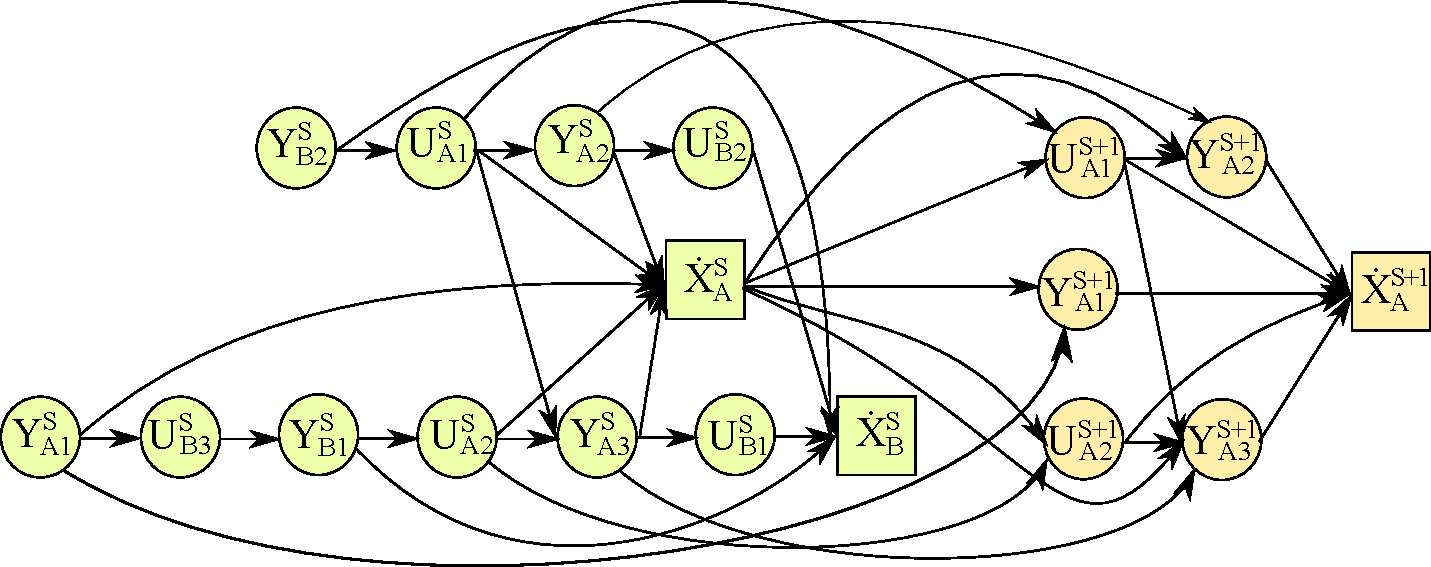
\includegraphics[scale=0.5]{figures/Operation_Graph_Two_Models_Multirate}
\caption{Graph obtained by applying the multi-rate transformation algorithm on the graph of Figure~\ref{fig:dag}}
\label{fig:dagmr}
\end{figure}

Without any loss of generality, the superscript which denotes the number of the occurrence of an operation is not used in the remainder of the thesis for the sake of simplicity, unless needed to specify the occurrence. Each occurrence of an operation $o_i^p$ in the graph $G(V,A)$ becomes an operation that is referred to using the notation $o_j$.

\section{Dependence Graph with Mutual Exclusion Constraints}
The FMI standard states that \textit{``FMI functions of one instance don't need to be thread safe''}. Therefore, an FMU does not implement any service to support concurrent access to its functions from multiple threads, and it is up to the executing environment to ensure the calling sequences of the FMU functions are respected as specified in the FMI standard. These restrictions introduce mutual exclusion constraints on the operations of the same FMU. We propose in this section an offline method for handling these constraints with low synchronization overhead.

\subsection{Motivation}

In order to study the impact of mutual exclusion constraints, we have evaluated the performance obtained using two mutual exclusion strategies. In the first one, a dedicated lock (system object that guarantees mutual exclusion) is used for each FMU. Every time an FMU function call is made at runtime, the associated lock has to be acquired before the execution of the function code can be started. This mechanism allows the synchronization of threads that execute different functions of the same FMU sharing same resources. Thanks to using the locks, each operation can be allocated to any core. We refer to such allocation as \textit{unconstrained allocation}. The second solution is explained in \cite{benkhaled:2014} and consists in allocating the operations of a same FMU to the same core. We refer to such allocation as \textit{constrained allocation}. The scheduling heuristic that was used in these tests is presented in Chapter \ref{ch:5-sched}. The theoretical speed-up was estimated by computing the makespan of the operation graph. The makepsan is the total time needed to compute the whole graph. Results are given in Figure \ref{fig:theoretical-speedup}. It shows that the expected speed-up using constrained allocation is less than the one using unconstrained allocation, when the number of cores is less than five, but similar when five cores or more are available. When using less than five cores, the large number of output operations can be efficiently allocated only if the unconstrained allocation is used: the speed-up difference between the constrained and the unconstrained allocation cases is due to this restriction on the allocation. Five is the minimal number of cores for enabling the execution of each state operation on a different core. Due to the predominant execution times of the state operations, their impact on the speed-up overrides the optimization of the allocation of the other operations. This explains why the speed-up difference between the unconstrained and the constrained allocation cases becomes very small using five cores or more.

\begin{figure}[phbt]
\centering
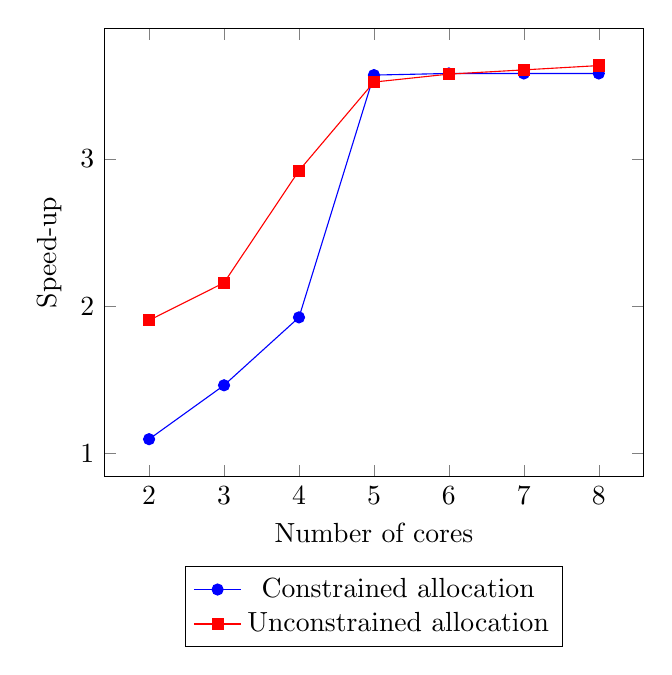
\begin{tikzpicture}
    \begin{axis}[
        xlabel=Number of cores,
        ylabel=Speed-up,legend style={at={(0.5,-0.2)},anchor=north}]
    \addplot[mark=*,blue,label=const] plot coordinates {
        (2,     1.097909998)
        (3,    1.463604418)
        (4,    1.924422442)
        (5,   3.568543452)
        (6,   3.579496624)
        (7,   3.579496624)
        (8,  3.579496624)
    };
    \addlegendentry{Constrained allocation}

    \addplot[color=red,mark=square*,label=unconst]
        plot coordinates {
        (2,     1.904310908)
        (3,    2.15962963)
        (4,   2.91987982)
        (5,   3.521135266)
        (6,  3.575107296)
        (7,  3.603831891)
        (8,  3.633021807)
        }; 
    \addlegendentry{Unconstrained allocation}
    \end{axis}
\end{tikzpicture}
\caption{Theoretical speed-up.}
\label{fig:theoretical-speedup}
\end{figure}

We implemented and tested both mutual exclusion strategies in order to compare their runtime performance. Tests were performed on the industrial use case described in Chapter \ref{ch:6-eval}. Execution times measurements were performed by getting the system time stamp at the beginning of the execution and after $30$ seconds of the simulated time. As previously mentioned, we compared the speed-up by dividing the single-core co-simulation execution time by the co-simulation execution time on a fixed number of cores. Figure \ref{fig:real-speedup} sums up the results. It shows the impact of mutex synchronization overhead on the speed-up. Whatever the number of the available cores, the speed-up remains close to $1.3$. On the contrary, the implementation of the constrained allocation results in a runtime speed-up that is similar to the theoretical speedup in terms of speed-up improvement when the number of cores is increased until reaching five. Nevertheless, the maximum measured speed-up ($2.4$) remains smaller than the theoretical one ($3.5$). In fact, the theoretical speed-up computation considers the makespan ratio without any estimation of the runtime overhead which certainly has an important impact on the speed-up.


\begin{figure}[phbt]
\centering
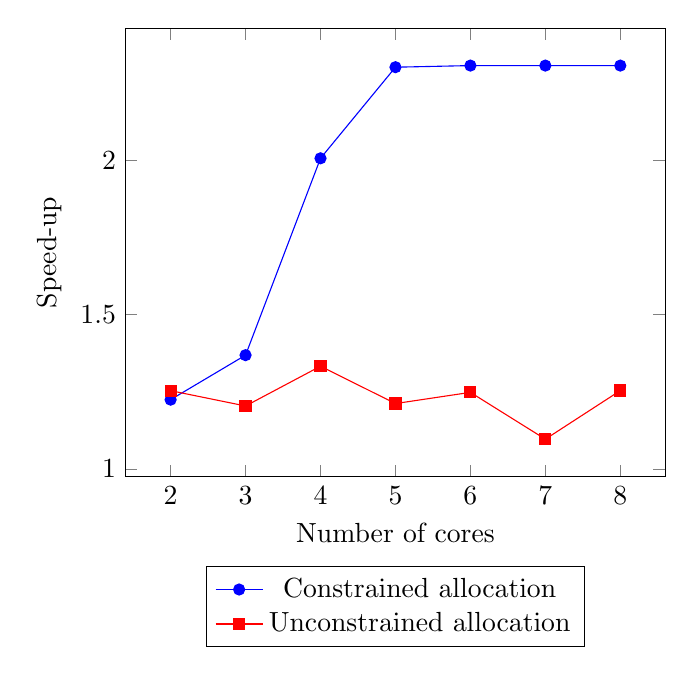
\begin{tikzpicture}
    \begin{axis}[
        xlabel=Number of cores,
        ylabel=Speed-up,legend style={at={(0.5,-0.2)},anchor=north}]
    \addplot[mark=*,blue,label=const] plot coordinates {
        (2,     1.223967163)
        (3,    1.368187328)
        (4,    2.005976773)
        (5,   2.301174325)
        (6,   2.306397786)
        (7,   2.306397786)
        (8,  2.306397786)
    };
    \addlegendentry{Constrained allocation}

    \addplot[color=red,mark=square*,label=unconst]
        plot coordinates {
        (2,     1.253126949)
        (3,    1.203511837)
        (4,   1.332430943)
        (5,   1.211351319)
        (6,  1.247650948)
        (7,  1.095957175)
        (8,  1.253420685)
        }; 
    \addlegendentry{Unconstrained allocation}
    \end{axis}
\end{tikzpicture}
\caption{Runtime speed-up.}
\label{fig:real-speedup}
\end{figure}

%The obtained results show the importance of employing a mutual exclusion strategy that is efficient with regards to the limitations of allocating the operations and the introduced synchronization overhead. In the rest of this section, we attempt to attain this objective.

The restrictions introduced by employing the tested mutual exclusion techniques makes it highly desirable to find an alternative solution that could satisfy the mutual exclusion constraints while: \begin{inlinelist} \item leaving as much flexibility as possible for allocating the operations to the cores and; \item introducing lower synchronization overhead \end{inlinelist}. In the rest of this section, we suggest a method for offline handling of mutual exclusion constraints. The proposed method is based on modeling the mutual exclusion constraints in the operation graph of the co-simulation.

\subsection{Acyclic Orientation of Mixed Graphs}

The operation graph model can be extended in order to represent scheduling problems that involve precedence constraints and also mutual exclusion constraints. This is commonly done using \textit{mixed graphs}. A mixed graph $G(V,A,D)$ is a graph which contains a set $A$ of directed arcs denoted $(o_i,o_j): 0 \leq i, j < n$ and a set $D$ of undirected edges denoted $[o_i,o_j]: 0 \leq i, j < n$. In the scheduling literature, these graphs are known also as \textit{disjunctive graphs} \cite{balas:1969}. In addition to the precedence constraints represented by arcs as described in Section \ref{sec:4-depgrph}, mutual exclusion relations are represented by edges in a mixed graph such that: 
\begin{itemize}
\item \textit{Precedence constraints:} $\forall (o_i,o_j) \in A, o_i$ must finish its execution before $o_j$ can start its execution.  
\item \textit{Mutual exclusion constraints:} $\forall [o_i,o_j] \in D, o_i$ and $o_j$ must be executed in strictly disjoint time intervals.
\end{itemize}

Operations belonging to the same FMU can be executed in either order but not in parallel. Undirected edges can be added between these operations in order to represent such mutual exclusion constraints. This transforms the operation graph into a mixed graph. In order to compute a schedule for such mixed graph, an execution order has to be defined for each pair of operations connected by an undirected edge which is interpreted by assigning a direction to this edge. Cycles must not be introduced in the graph while assigning directions to edges, otherwise, the scheduling problem becomes infeasible. Once all edges have been assigned directions, the result is a new operation graph which is a DAG.
Since the final goal is to accelerate the execution of the co-simulation which comes down to minimizing the makespan of the operation graph, the acyclic orientation of the mixed graph has to minimize the length of the critical path of the resulting DAG. We recall that the length of the critical path of the operation graph represents a lower bound on the makespan of the graph. This problem is known as \textit{acyclic orientation} \cite{barbosa:1999}. We denote the acyclic orientation as a function $\phi:\ {[o_i,o_j] \in D} \rightarrow \{(o_i,o_j),(o_j,o_i)\}$

%\subsubsection{Graph Coloring of Undirected Graphs}
% Talk about Gallai–Hasse–Roy–Vitaver theorem
The acyclic orientation problem is closely related to vertex coloring of a graph \cite{jensen:2011}. In its general form, i.e. when all edges of the graph are undirected, vertex coloring is a function $\alpha: V \rightarrow \{1, 2, \ldots, k\}$ which labels the vertices of the graph with integers, called colors, such that the inequality \ref{eq:color1} holds.

\begin{equation}
\forall\ [o_i,o_j] \in D,\ \alpha(o_i) \neq \alpha(o_j)
\label{eq:color1}
\end{equation}

The acyclic orientation of the graph can then be obtained by assigning a direction to every edge such that the color of the corresponding tail vertex is smaller than the color of the corresponding head vertex. A graph coloring with $k$ colors is referred to as \textit{k-coloring}. In its general form, vertex coloring aims at finding a \textit{minimum vertex coloring}, i.e. minimizing $k$ the number of the used colors. The minimum number of colors required to color an undirected graph $G$ is called the chromatic number and is denoted $\chi(G)$. The Gallai–Hasse–Roy–Vitaver theorem \cite{gallai:1968,roy:1967,hasse:1966,vitaver:1962} links the length of the longest path of the graph, obtained by the orientation which minimizes this length, to vertex coloring of the graph. It states that the length of the longest path of a directed graph is at least $\chi(G)$. Thus, a minimum vertex coloring leads to an acyclic orientation that minimizes the length of the critical path of the resulting graph. Computing the chromatic number of a graph is NP-complete.

The acyclic orientation of a mixed graph can be obtained via vertex coloring also. However, vertex coloring of a mixed graph has to take into account both arcs and edges of the graph. More precisely, a vertex coloring of a mixed graph is a function $\alpha: V \rightarrow \{1, 2, \ldots, k\}$ such that inequalities \ref{eq:color1} and \ref{eq:color2} hold.

\begin{equation}
\forall\ (o_i,o_j) \in A,\ \alpha(o_i) < \alpha(o_j)
\label{eq:color2}
\end{equation}

A coloring of a mixed graph $G(V,A,D)$ exists only if it is cycle-free \cite{ries:2007}, i.e. the directed graph $G(V,A,\emptyset)$ does not contain any cycle. The problem of acyclic orientation of mixed graphs has been studied in the literature in \cite{andreev:2000,sotskov:2002,al-anzi:2006}. Efficient algorithms have been proposed for the orientation of special types of mixed graphs. It has been shown that, in the general case, the problem is NP-Hard.

\subsection{Problem Formulation}

Let $G(V,A)$ be an operation graph of an FMU co-simulation constructed as described in Section \ref{sec:4-depgrph}. In order to represent mutual exclusion constraints between FMU operations, the initial operation graph $G(V,A)$ is transformed into a mixed graph by connecting each pair of mutually exclusive operations $o_i, o_j$ by and edge $[o_i, o_j]$. The resulting mixed graph is denoted $G(V,A,D)$, where $V$ is the set of operations, $A$ is the set of arcs, and $D$ is the set of edges. Once the mixed graph is constructed, directions have to be assigned to its edges in order to define an order of execution for mutually exclusive operations. The precedence and mutual exclusion relations represented by the mixed graph $G(V,A,D)$ are given by expressions \ref{eq:color4} and \ref{eq:color5} respectively. If operations $o_i$ and $o_j$ are connected by an arc $(o_i,o_j)$, the time interval $(S(o_i), E(o_i)]$ must precede the time interval $(S(o_j), E(o_j)]$. Otherwise, if operations $o_i$ and $o_j$ are connected by an edge $[o_i,o_j]$, time intervals $(S(o_i), E(o_i)]$ and $(S(o_j), E(o_j)]$ must be strictly disjoint.

\begin{equation}
\forall\ (o_i,o_j) \in A,\ E(o_i) \leq S(o_j)
\label{eq:color4}
\end{equation}

\begin{equation}
\forall\ [o_i,o_j] \in D,\  (S(o_i), E(o_i)] \cap (S(o_j), E(o_j)] = \emptyset
\label{eq:color5}
\end{equation}

The timing attributes of the operations in the mixed graph $G(V,A,D)$ are the same as in the initial graph $G(V,A)$ because the added set of edges $[o_i, o_j] \in D$ does not impact the computation of these attributes. The attributes of an operation $o_i$, connected by an edge with another operation, may change only when this edge is assigned a direction following the order of the execution intervals of $o_i$ and $o_j$. 

An edge $[o_i,o_j]$ is called a conflict edge if the intervals $(S(o_i), E(o_i)]$ and $(S(o_j), E(o_j)]$ in the graph $G(V,A)$ overlap. This can be written in the form of expression \ref{eq:conflict}. If for a given edge $[o_i,o_j]$ either $E(o_i) \leq S(o_j)$ or $E(o_j) \leq S(o_i)$, there is no conflict and the edge can be assigned a direction. 

\begin{equation}
E(o_i) > S(o_j)\ \text{and}\ E(o_j) > S(o_i)
\label{eq:conflict}
\end{equation}

It should be noted that, for a given edge $[o_i, o_j]$, choosing either of the execution orders does not impact the numerical results of the co-simulation since these operations do not have data dependence. An order have to be defined only because we have to ensure mutual exclusion between them due to the non-thread-safe implementation of FMI. Following the definition given in the previous section, the corresponding vertex coloring is a function $\alpha: V \rightarrow \{1, 2, \ldots, k\}$ which is equivalent to mapping the operations $o_i \in V$ to the time intervals $[S(o_1), E(o_1)], [S(o_2), E(o_2)], \ldots, [S(o_n), E(o_n)]$.

The problem of acyclic orientation of the mixed graph $G(V,A,D)$ can be stated as an optimization problem as follows:

\begin{itemize}[label={},topsep=1pt,parsep=1pt,partopsep=1pt,leftmargin=*]	
\item \textbf{Input:} Mixed graph $G(V,A,D)$
\item \textbf{Output:} DAG $G(V,A)$
\item \textbf{Find:} Coloring $\alpha: V \rightarrow \{1, 2, \ldots, k\}$
\item \textbf{Minimize:} Number of colors $k$
\item \begin{subjecto}
			      \item $\forall\ (o_i,o_j) \in A,\ \alpha(o_i) < \alpha(o_j)$
				   	\item $\forall\ [o_i,o_j] \in D,\ \alpha(o_i) \neq \alpha(o_j)$
       \end{subjecto}
\end{itemize}

%This formulation is stated as a vertex coloring problem, however, it is possible to state the problem using either vertex coloring notation or scheduling notation. Thus, we note the following equivalence:
%
%\begin{itemize}[label={},topsep=1pt,parsep=1pt,partopsep=1pt,leftmargin=*]	
%\item Coloring $\alpha: V \rightarrow \{1, 2, \ldots, k\} \equiv$ Scheduling $\alpha: V \rightarrow \{[S(o_1), E(o_1)],$ $[S(o_2), E(o_2)],$ $\ldots,$ $[S(o_n), E(o_n)]\} \equiv$ Assignment $\alpha: D \rightarrow \{(o_i,o_j),(o_j,o_i): [o_i,o_j] \in D\}$
%\item $\forall\ (o_i,o_j) \in A,\ \alpha(o_i) < \alpha(o_j) \equiv \forall\ (o_i,o_j) \in A,\ E(o_i) \leq S(o_j)$
%\item $\forall\ [o_i,o_j] \in D,\ \alpha(o_i) \neq \alpha(o_j)$ $\equiv$ $\forall\ [o_i,o_j] \in D,\  (S(o_i), E(o_i)] \cap (S(o_j), E(o_j)] = \emptyset$
%\item Optimal coloring $min(k)$ $\equiv$ Optimal length of the critical path $min(R)$
%\end{itemize}

\subsection{Resolution using Integer Linear Programming}

Let $G(V,A,D)$ be a mixed graph constructed form the operation graph $G(V,A)$ as described in the previous sections to represent precedence and mutual exclusion constraints between operations of an FMU co-simulation. In the following, we present an Integer Linear Programming formulation for the problem of acyclic orientation of $G(V,A,D)$. The proposed formulation is based on the scheduling notation which gives a more compact set of constraints compared to a formulation that uses the vertex coloring notation.

\subsubsection{Variables and Constants}

Tables \ref{table:varilporient} and \ref{table:consilporient} summarize the variables and the constants that are used in the ILP formulation respectively.

\begin{table}[!htbp]
\caption{Variables used in the ILP formulation of the acyclic orientation problem}
\centering
\label{table:varilporient}
\begin{tabular}{l l l}
\toprule
Variable & Type & Description  \\
\midrule
 $S(o_i)$ & Integer & Start time of operation $o_i$\\
 $E(o_i)$ & Integer & End time of operation $o_i$\\
 $b_{ij}$ & Binary & Orientation decision variable associated with edge $[o_i,o_j] \in D$\\
 $CP$ & Integer & Length of the critical path of the graph\\
\bottomrule
\end{tabular}
\end{table}

\begin{table}[!htbp]
\caption{Constants used in the ILP formulation of acyclic orientation problem}
\centering
\label{table:consilporient}
\begin{tabular}{l l l}
\toprule
Constant & Type & Decription\\
\midrule
 $C(o_i)$ & Integer & Execution time of operation $o_i$\\
 $M$ & Integer & Large positive number\\
\bottomrule
\end{tabular}
\end{table}

\subsubsection{Constraints}

The following set of constraints is used in the ILP formulation of the acyclic orientation problem:

\begin{itemize}

\item \textit{Precedence constraints:} The start time of each operation is equal to the maximum of the end times of all its predecessors. Expression \ref{orient:const_1} captures this constraint. Note that expression \ref{orient:const_1} indicates that the start time of operation $o_j$ is greater or equal to the end time of each predecessor $o_i$. This is sufficient to express $S(o_j) = max_{o_i \in pred(o_j)}(E(o_i))$ since the formulated problem is a minimization problem.

\begin{equation}
\forall (o_i,o_j) \in A, S(o_j) \geq E(o_i)
\label{orient:const_1}
\end{equation}

\item \textit{Mutual exclusion constraints:} We define the binary variable $b_{ij}$ which is associated with the direction that is assigned to edge $[o_i,o_j]$. $b_{ij}$ is set to $1$ if the edge $[o_i,o_j]$ is assigned a direction from $o_i$ to $o_j$, i.e. $\phi([o_i,o_j]) = (o_i,o_j)$ and to $0$ otherwise. Note that $b_{ij}$ is the complement of $b_{ji}$. For every pair of operations that are connected by and edge, we have to ensure that their time intervals are strictly disjoint, i.e. $\forall\ [o_i,o_j] \in D,\  (S(o_i), E(o_i)] \cap (S(o_j), E(o_j)] = \emptyset$. Expressions \ref{orient:const_2} and \ref{orient:const_3} capture this constraint where $M$ is a large positive integer.

\begin{equation}
\forall [o_i,o_j] \in E, S(o_i) \geq E(o_j) - M \times (1-b_{ij})
\label{orient:const_2}
\end{equation} 

\begin{equation}
\forall [o_i,o_j] \in E, S(o_j) \geq E(o_i) - M \times b_{ij}
\label{orient:const_3}
\end{equation}

\item \textit{Time intervals:} Expression \ref{orient:const_4} is used to compute the end time of each operation.

\begin{equation}
\forall o_i \in V, E(o_i) = S(o_i) + C(o_i)
\label{orient:const_4}
\end{equation} 

\item \textit{Length of the critical path:} The critical path $CP$ is equal to the maximum of the end times of all the operations as stated by expression \ref{orient:const_5}.

\begin{equation}
\forall o_i \in V, P \geq E(o_i)
\label{orient:const_5}
\end{equation}

\end{itemize}

\subsubsection{Objective}

The objective of this linear program is to minimize the length of the critical path of the operation graph (expression \ref{orient:obj}).

\begin{equation}
min(P)
\label{orient:obj}
\end{equation}

While exact algorithms such as ILP give optimal results, they suffer form very long execution times that are not acceptable for the users. For many real world applications, ILP fails to produce the results within acceptable times. Heuristics are usually good alternatives. While the optimality of the solution cannot be guaranteed when using heuristics, they, in most cases, provide results of good quality, not too far form the optimal solution within acceptable execution times.

\subsection{Acyclic Orientation Heuristic}

We propose in this section a heuristic for the acyclic orientation of the mixed graph $G(V,A,D)$. A straightforward acyclic orientation can be obtained by sorting the operations in a non decreasing order of their start times $S(o_i)$ and assigning directions to edges following this order, i.e. $\forall [o_i,o_j] \in D, S(o_i) \leq S(o_j), \phi([o_i,o_j]) = (o_i,o_j)$. This is a fast greedy acyclic orientation, however it can be improved as we show hereafter.

Let $s$ be the sum of the repetition factors of all the FMUs. The set of operations $V$ can be represented as a union of mutually disjoint non empty subsets such that every subset contains all operations that belong to the same FMU and that correspond to the same occurrence:

\begin{equation}
V = \bigcup_{k=1}^s V_k:\ \forall\ o_i^p, o_j^q \in V_k,\ k \in \{0, 1, \ldots, s\},\ f_m(o_i^p)=f_m(o_j^q)\ \text{and}\ p = q
\label{eq:opsubset}
\end{equation}

We know that edges in the set $D$ exist only between operations that belong to the same FMU. Furthermore, for every edge $[o_i^p,o_j^q] \in D$, operations $o_i^p$ and $o_j^q$ correspond to the same occurrence, i.e. $p = q$. Although operations which belong to the same FMU and correspond to different occurrences are mutually exclusive, it is not needed to connect them by an edge because an execution order is already ensured for these operations by the way the operation graph is constructed. In other words, all the operations of an FMU, and which correspond to the same occurrence $p$ have to finish their execution before the next occurrence $p+1$ of any operation can start its execution. Similarly to the operation set, the edge set $D$ can be subdivided into mutually disjoint non empty subsets:

\begin{equation}
D = \bigcup_{k=1}^s D_k,\ \forall\ [o_i^p, o_j^q] \in D_k,\ k \in \{0, 1, \ldots, s\},\ f_m(o_i^p)=f_m(o_j^q)\ \text{and}\ p = q
\label{eq:opsubset}
\end{equation}

In view of the above, we define the set of subgraphs which constitute the graph $G(V,\emptyset,D) = \bigcup_{k=1}^s G(V_k,D_k)$. Theorem \ref{theorem:orient} states the relationship between the acyclic orientations of the subgraphs $G(V_k,D_k)$ and the acyclic orientation of the mixed graph $G(V,A,D)$.

\begin{theorem}
An acyclic orientation of the mixed graph $G(V,A,D)$ can be obtained by finding an acyclic orientation for every subgraph $G_k(V_k,D_k)$ following the non decreasing order of the start times of the operations as described previously.
\label{theorem:orient}
\end{theorem}

\begin{proof}
In order to prove this, we have to show that every edge in $D$ is assigned a	direction and that the resulting orientation does not lead to the creation of a cycle. We use a proof by contradiction to prove this statement. Since every edge $[o_i, o_j]$ belongs to one subset of edges $D_k$, finding acyclic orientations for all the subgraphs $G_k(V_k)$ leads to assigning a direction to every edge in $D$. The existence of a cycle in the resulting graph means that there exists at least an edge $[o_i,o_j]$, such that $S(o_i) > S(o_j)$, that has been transformed into the arc $(o_i,o_j)$. However, this is not possible because the greedy acyclic orientation assigns directions to edges following a non-decreasing order of the start times of the operations which contradicts the previous assertion and thus proves Theorem \ref{theorem:orient}.
\end{proof}

Consider now that the acyclic orientation of each subgraph $G_k(V_k,D_k)$ is obtained by finding a vertex coloring for this subgraph. This vertex coloring can be seen as a sequence of assignments $\alpha_1, \alpha_2, \ldots, \alpha_{|D_k|}$, such that every assignment $\alpha_l$ assigns a color to one operation $o_i \in V_k$ and leads to assigning directions to edges that connect $o_i$ with other already colored operations $o_j \in V_k$. The number of assignments needed to perform the acyclic orientation of $G_k(V_k,D_k)$ is at most equal to the number of edges $|D_k|$. Following the coloring of an operation and the engendered assignment of directions, the attributes of some operations may change. Two situations have to be distinguished:

\begin{itemize}
\item Coloring $\alpha_l$ of operation $o_i$ does not lead to assigning a direction to any conflict edge. In this case, no changes of the timing attributes occur.
\item Coloring $\alpha_l$ of operation $o_i$ leads to assigning a direction to at least one conflict edge $[o_i,o_j] \in D_k$. Without any loss of generality, suppose that the edge $[o_i,o_j]$ is transformed into the arc $(o_i,o_j)$. The start time $S(o_j)$ is changed as follows: $S(o_j) \leftarrow E(o_i)$. This leads to changing the end time $E(o_j)$ also and possibly causes a domino effect for the start times and end times of all the descendants $o_{j'} \in desc(o_j)$ (see Algorithm \ref{algo:update_s}). Moreover, if $\overline{S}(o_j) > \overline{E}(o_i)$, the end time from end $\overline{E}(o_i)$ is changed as follows: $\overline{E}(o_i) \leftarrow \overline{S}(o_j)$. Similarly, this leads to changing the start time from end $\overline{S}(o_j)$ and possibly causes a domino effect for the start times and end times of all the ancestors $o_{i'} \in ance(o_i)$ (see Algorithm \ref{algo:update_e}).
\end{itemize}

\begin{algorithm}[htb]
	\SetKwFunction{update}{update}
	\SetKwInOut{Input}{Input}
  \SetKwInOut{Output}{Output}
	\Input{Attributes of the mixed graph $G(V,A,D)$, partially colored subgraph $G_k(V_k,A_k,D_k)$\;}
	\Output{Update of the start and end times of a subset of operations $\{o_i\} \subset V$\;}
	Set $\alpha_l$ the last assignment of color made to an operation $o_i \in V_k$\;
	Set $A_{k,l} = \{(o_t,o_h)\}$ the set of all arcs created from the orientations engendered by $\alpha_l$\;
	\ForEach{$(o_t,o_h) \in A_{k,l}$}
		{
			\If{$S(o_h) < E(o_t)$ and $S(o_t) < E(o_h)$}
				{
					$S(o_h) \leftarrow E(o_t)$\;
					$E(o_h) \leftarrow S(o_h) + C(o_h)$\;
					\update{$o_h$}\;
				}
		}
	\SetKwProg{myproc}{Procedure}{}{}
	\myproc{\update{$o_h$}}
		{
			\If{$succ(o_h) \neq \emptyset$}
			{
				\ForEach{$o_{h'} \in succ(o_h)$}
						{
							\If{$S(o_{h'}) < E(o_h)$}
							{
								$S(o_{h'}) \leftarrow E(o_h)$\;
								$E(o_{h'}) \leftarrow S(o_{h'}) + C(o_{h'})$\;
								\update{$o_{h'}$}\;
							}
						}
			}
			 \KwRet\;
		}
	\caption{Update of the start and end times following an assignment $\alpha_l$}
	\label{algo:update_s}
\end{algorithm}


\begin{algorithm}[htb]		
	\SetKwFunction{update}{update}
	\SetKwInOut{Input}{Input}
  \SetKwInOut{Output}{Output}
	\Input{Input Attributes of the mixed graph $G(V,A,D)$, partially colored subgraph $G_k(V_k,A_k,D_k)$\;}
	\Output{Output Update of the start and end times from end of a subset of operations $\{o_i\} \subset V$\;}
	Set $\alpha_l$ the last assignment of color made to an operation $o_i \in V_k$\;
	Set $A_{k,l} = \{(o_t,o_h)\}$ the set of all arcs created from the orientations engendered by $\alpha_l$\;
	\ForEach{$(o_t,o_h) \in A_{k,l}$}
		{
			\If{$S(o_h) < E(o_t)$ and $S(o_t) < E(o_h)$}
				{
					\If{$\overline{E}(o_t) < \overline{S}(o_h)$}
						{
							$\overline{E}(o_t) \leftarrow \overline{S}(o_h)$\;
							$\overline{S}(o_t) \leftarrow \overline{E}(o_t) + C(o_t)$\;
							\update{$o_t$}\;
						}
					
				}
		}
	\SetKwProg{myproc}{Procedure}{}{}
	\myproc{\update{$o_t$}}
		{
			\If{$pred(o_t) \neq \emptyset$}
			{
				\ForEach{$o_{t'} \in pred(o_t)$}
						{
							\If{$\overline{E}(o_t^*) < \overline{S}(o_t)$}
							{
								$\overline{E}(o_{t'}) \leftarrow \overline{S}(o_t)$\;
								$\overline{S}(o_{t'}) \leftarrow \overline{E}(o_{t'}) + C(o_{t'})$\;
								\update{$o_{t'}$}\;
							}
						}
			}
			 \KwRet\;
		}
	\caption{Update of the start and end times from end following an assignment $\alpha_l$}
	\label{algo:update_e}
\end{algorithm}

We now describe our proposed acyclic orientation heuristic. The heuristic takes as input a mixed graph $G(V,A,D)$ and the attributes of the operations $o_i \in V$ as computed for the digraph $G(V,A,\emptyset)$, and assigns directions to all the edges $[o_i,o_j] \in D$. By applying Theorem \ref{theorem:orient}, the heuristic consists in finding vertex colorings of the subgraphs which constitute the graph $G(V,A,D)$. 
In the first step, the graph $G(V,\emptyset,D)$ obtained by removing all the arcs $(o_i,o_j) \in A$ from the mixed graph $G(V,A,D)$ is partitioned into $s$ subgraphs where $s$ is the sum of the repetition factors of all FMUs such that each subgraph contains all the operations of one FMU which correspond to the same occurrence and all the edges that connect them: $ G(V,\emptyset,D)= \bigcup_{k=1}^s G_k(V_k,\emptyset,D_k)$. Then, the set of operations $o_i \in V$ is sorted in a non decreasing order of the start times $S(o_i)$. Next, the heuristic iteratively assigns colors to operations. 
It keeps a list of of already colored operations $L_k$ for each subgraph $G(V_k,\emptyset,D_k)$. The operations of every list $o_i \in L_k$ are sorted in increasing order of their assigned colors. At each iteration, the heuristic selects among the operations not yet colored $o_i \in V$, the operation which has the earliest start time $S(o_i)$ to be assigned a color. Ties are broken by selecting the operation with the least flexibility. We call the operation to be colored at a given iteration, the \textit{pending operation}. The heuristic checks in the order of $L_k$ if the edges which connect the pending operation $o_i \in V_k$ with the operations $o_j \in L_k$ are conflict edges. 
If a conflict edge $[o_i,o_j] \in D_k: o_j \in L_k$ is detected, the pending operation is assigned the color $\alpha(o_j)$ and the colors assigned to all the already colored operations $o_{i'} \in L_k:\ \alpha(o_{i'}) \geq \alpha(o_{i})$, are increased $\alpha(o_{i'}) \leftarrow \alpha(o_{i'})+1$. The corresponding edges are then accordingly assigned directions. Afterward, the timing attributes of the operations are updated using Algorithms \ref{algo:update_s} and \ref{algo:update_e}. At this point, the increase in $CP$, the critical path of the graph, is evaluated. Next, the operations $o_{i'} \in L_k$: $\alpha(o_{i'}) > \alpha(o_{i})$ are reassigned their previous colors $\alpha(o_{i'}) = \alpha(o_{i'})-1$, and the pending operation is assigned a new color $\alpha(o_i) \leftarrow \alpha(o_i)+1$. The increase in the critical path is evaluated again similarly. After repeating this process for all the edges $[o_i,o_{i'}] \in D_k:\ o_{i'} \in L_k$, the pending operation is finally assigned the color which leads to the least increase in the critical path, and edges $[o_i,o_{i'}] \in D_k : o_i' \in L_k$ are assigned directions accordingly. The heuristic begins another iteration by selecting a new operation to be colored. The heuristic assigns a color to one operation at each iteration. Every operation is assigned a color higher than the colors of all its predecessors which guarantees that no cycle is generated. The heuristic finally stops when all the operations have been assigned colors. 
%Dont forget to add case not conflict edge
\begin{algorithm}[!htp]
	\SetKwFunction{evaluate}{evaluate}	
	\SetKwInOut{Input}{Input}
  \SetKwInOut{Output}{Output}
	\Input{Mixed graph $G(V,A,D)$}
	\Output{DAG $G(V,A)$\;}
	Set $s$ the number of all occurrences of all FMUs\;
	Partition the graph $G(V,\emptyset,D)$ into $s$ subgraphs: $ G(V,\emptyset,D)= \bigcup_{k=1}^s G_k(V_k,\emptyset,D_k)$\;
	Initialize lists $L_k \leftarrow \emptyset: 0 \leq k < s$\;
	Set $\Omega$ the set of all the operations not already colored\;
	\While{$\Omega \neq \emptyset$}
	{
		Select the operation $o_i \in V_k:\ S(o_i) = \max_{o_j \in \Omega}(S(o_j)), 0 \leq k < s$ (break ties by selecting the operation with the least flexibility)\;
			\If{$L_k = \emptyset$}
			{
				$\alpha(o_i) \leftarrow 1;\ L_k \leftarrow L_k \cup \{o_i\}$\;
			}
		\Else
		{
		Set $\sigma \leftarrow \infty$; \tcp{Initialize the increase in the critical path}
		\ForEach{$o_j \in L_k$}
		{
				\If{$S(o_i) < E(o_j)$ and $S(o_j) < E(o_i)$}
				{
				\ForEach{$c \in \{\alpha(o_j), \alpha(o_j)+1\}$ }
			   {
					$\alpha(o_i) \leftarrow c$\;
					\evaluate{$o_i, L_k$}\;
					\ForEach{$o_{i'} \in L_k$: $\alpha(o_{i'}) > \alpha(o_i)$}
							{
								Reassign $o_{i'}$ its previous color: $\alpha(o_{i'}) \leftarrow \alpha(o_{i'})-1$\;
							}
					}
				}
				\If{$S(o_i) \geq E(o_j)$}
				{
					$\alpha(o_i) \leftarrow \alpha(o_j)+1$\;
					\evaluate{$o_i, L_k$}\;
				}
				\Else
				{
					$\alpha(o_i) \leftarrow \alpha(o_j)$\;
					\evaluate{$o_i, L_k$}\;
				}
			
			$\alpha(o_i)=color$\;
			\ForEach{$o_{i'} \in L_k$}
			{
				\If{$\alpha(o_{i'}) > \alpha(o_i)$}
				{
					Assign a direction to the edge $[o_i,o_{i'}] \in D_k: \phi([o_i,o_{i'}])\leftarrow (o_i,o_{i'})$\;
				}
				\Else
				{
					Assign a direction to the edge $[o_i,o_{i'}] \in D_k: \phi([o_i,o_{i'}])\leftarrow (o_{i'},o_i)$\;
				}
			}
			Update the timing attributes using Algorithms \ref{algo:update_s} and \ref{algo:update_e}\;
			Remove $o_i$ from $\Omega;\ L_k \leftarrow L_k \cup \{o_i\}$\;
		}
		}
	}
	\SetKwProg{myproc}{Procedure}{}{}
	\myproc{\evaluate{$o_i, L_k$}}
		{
			 \ForEach{$o_{i'} \in L_k:\ \alpha(o_{i'}) \geq \alpha(o_i)$}
						{
							
								$\alpha(o_{i'}) \leftarrow \alpha(o_{i'}) + 1$\;
								Update the timing attributes using Algorithms \ref{algo:update_s} and \ref{algo:update_e}\;
						}
						Compute the new critical path and set $\sigma'$ the increase in the critical path\;
						\If{$\sigma' < \sigma$}
							{
								$color \leftarrow \alpha(o_i);\ \sigma \leftarrow \sigma'$\;
							}
			 \KwRet\;
		}
 
	\caption{Acyclic orientation heuristic}
	\label{algo:ao}
\end{algorithm}

\subsubsection{Complexity}

The outermost loop (while loop) of the acyclic orientation heuristic is repeated $n$ times, such that at each iteration, one operation is assigned a color. Recall that $n$ is the number of operations in the operation graph $G(V,A)$. The selection of the operation with latest start time is done in $\mathcal{O}(\log{}n)$. The first inner loop iterates over all the edges connecting the selected operation. It is repeated at most $e$ times, where $e$ is the maximum number of edges connecting one operation. The inner most loop is executed twice in all cases. This results in an execution of the nested inner loops in $O(e)$. In addition Algorithms \ref{algo:update_s} and \ref{algo:update_e} that are called in the heuristic have each a complexity of $O(n)$ since they are based on a recursion whose depth is at most $n$. Therefore, the complexity of the acyclic orientation heuristic is evaluated to $\mathcal{O}(n^2e)$.  


%\subsubsection{Soundness}
%
%\subsubsection{Completeness}
%
%\subsubsection{Termination}

\section{\label{sec:grphrtsc}Dependence Graph with Real-time Constraints}

Real-time (co-)simulation, a widely used term in the literature, refers to co-simulation that requires that the amount of time needed to compute all equations of a model must be less than the integration step size of the model \cite{belanger:2010}. In this thesis, we talk instead about \textit{co-simulation under real-time constraints}. The difference between the two notions will be clarified through this section. In particular, we are interested in such co-simulation within the context of HiL testing. In this section, we focus on defining these real-time constraints which are not given as it is usually the case in classical real-time systems. First, we explain what these constraints are and where they originate from. Then, we describe how to define real-time constraints for a co-simulation represented by an operation graph. The work presented in this section is based on the method of propagating real-time constraints described in \cite{faure:2011}. This method was proposed for co-simulations where only partial information about intra-model dependence is available. Our work is an adaptation of this method to FMU co-simulation represented by a dependence graph which provides information about input/output/state dependence.

\subsection{Preliminaries}

A HiL setup is composed of a simulated component and a physically available component that is interfaced with the simulated component via inputs and outputs. It should be noted that multiple parts may be physically available and involved in HiL, e.g. multiple controllers interacting with multiple parts of physical processes. We refer to all these parts as the real component. Figure \ref{fig:hilSetup} shows a basic example of a HiL co-simulation. The simulated component is represent by an operation graph. It consists of two FMUs $A$ and $B$ whose operations are colored in green and yellow respectively. The real component has one input and one output connected to an output operation and and an input operation of the simulated component respectively. 

\begin{figure}[phbt]
\centering
\includestandalone{figures/hilsetup}
\caption{Example of co-simulation under real-time constraints.}
\label{fig:hilSetup}
\end{figure}

The goal of the HiL testing phase in the model based design process is mainly to run realistic tests. In other words, it aims at estimating the performance of the real component by providing a realistic environment through the simulated component. The simulated component has to interact with the real component at the same rate as its real counterpart. As such, the inputs and outputs of the real component, which are periodically sampled, define real-time constraints which involve that the simulated time has to match the real time. These constraints are initially defined on the outputs and inputs of the simulated component that are connected with the inputs and outputs of the real component respectively. Since these inputs and outputs of the simulated component depend on other operations of the co-simulation, the real-time constraints are propagated towards the other operations.

In \cite{faure:2011}, it has been shown that the real-time constraints have to be propagated in different ways depending on the type of the operation (input, output, state) and also the type of intra-model connections (direct feedthrough, non direct feedthrough). In this work, the author dealt with co-simulation at the model level, i.e. a co-simulation is represented by a graph of models. Moreover, the author distinguishes between direct feedthrough and non direct feedthrough model. A direct feedthrough model contains at least one output which directly depends on an input while a non direct feedthrough models contains none. For further details, one should consult the original work. Because we adopted a different approach which takes advantage of the FMI standard to represent a co-simulation with finer granularity, we cannot apply the method proposed in \cite{faure:2011}. Instead, we propose a new method that we present in this section. First, we give in the following some preliminaries about the propagation of real-time constraints on a dependence graph representing an FMU co-simulation. 

Different hardware and software components such as communication buses and software acquisition modules are used to connect the real component with the simulated component (co-simulation). In our work, we abstract the details about all these communication components away by representing the connection as a data dependence between an input (resp. output) of the real component and an output (resp. input) of the co-simulation (see Figure \ref{fig:hilSetup}). The co-simulation periodically reads and writes data from and to the real component. Therefore, the real-time constrainsts are initially defined on the inputs and outputs that are directly connected with the real component. For instance, the real component sends data via its output to update an input of the co-simulation every $20ms$.

We consider that the simulated component consists in an FMU co-simulation represented as an operation graph constructed and upon which the different transformations (multi-rate, acyclic orientation) have been applied as described in previous sections. All operations of the co-simulation including the inputs (resp. outputs) of the co-simulation that are connected with the real component may have successors or not. This is an important difference from the method proposed in \cite{faure:2011} where outputs of the co-simulation do not have successors. 

We assume that the sampling period of a given input/output of the real component is a multiple of the communication step size of the operation of the simulated component that is connected with it. In contrast to \cite{faure:2011}, we do not consider the case where cycles exist in the operation graph since, as we showed previously, the operation graphs we deal with are cycle-free by construction. 

The propagation of real-time constraints loosens the constraints imposed on the co-simulation compared to classical real-time co-simulation \cite{belanger:2010}. The latter, indeed, requires setting a periodic deadline for the computations of each model's equations that is equal to its integration step size. This approach, in the case of HiL co-simulation where only data exchange between the real and the simulated component have to be performed in real-time, usually over-constrains the co-simulation. We chose to use the term co-simulation under real-time constraints over the term real-time co-simulation because, in our approach, not every operation is constrained to be executed in real-time, i.e. with a periodic deadline that is equal to its integration step size. In the subsequent sections, we present how the real-time constraints are computed and propagated. %We consider special cases of operation graphs and present how they can be handled.

\subsection{Definition of Real-time Constraints}

Real-time systems are based on real-time tasks which represent the elementary units of execution. These tasks are characterized by a number of parameters such as periods, Worst Case Execution Times (WCET), deadlines, and release dates. Such parameters constitute an abstract model of the tasks that is used for the design and the analysis of real-time systems. We consider co-simulation under real-time constraints to be a real-time system where the operations of the co-simulation represent the real-time tasks. Therefore, the operation graph model presented in \ref{sec:4-depgrph} has to be completed with real-time parameters that will allow the design and the analysis of real-time multi-core scheduling algorithms for co-simulation under real-time constraints. Hereinafter, we define real-time constraints that are assigned to operations, necessary for performing HiL co-simulation.

Let the inputs and the outputs of the real component be sampled with sampling periods $T_{x}$  and $T_{y}$ respectively where $x$ and $y$ denote the numbers of the corresponding input and output respectively. In other words, an input (resp. output) of the real component is periodically activated every $T_{x}$ (resp. $T_{y}$) units of time. The sampling periods of the different inputs and outputs of the real component can be identical or different.% In this work, we assume that every sampling period is a multiple of the communication step sizes of the simulated FMUs. Otherwise, the hardware may miss some of the values provided by the simulated part and vice versa.
 We refer to operations of the simulated component that are directly connected to the real component as \textit{gate operations}, e.g. operations $o_4$ and $o_5$ in Figure \ref{fig:hilSetup}.  

The periodic activation of an output of the real component leads to producing data that are consumed by an input gate operation $o_i$ of the simulated component. This input gate operation is periodically updated by the values produced by the output of the real component following a sampling period $T_{y}$. Therefore, at the $z^{th}$ sample $z \times T_{y}$, the input gate operation $o_i$ is updated to its value corresponding to simulated time $z \times T_{y}$. This defines a periodic release for this input gate operation, i.e. time points at which its value is periodically updated following consumption of data produced by the real component.

\begin{definition}
A \textit{release} is a real-time constraint applied on an input gate operation $o_i$ of the simulated component in a HiL co-simulation. Such constraint is defined by its period $R(o_i) = T_{y}$ where $T_{y}$ is the sampling period of the output of the real component that is connected with $o_i$. The occurrences of a release constraint are written $z \times T_{y}, z \in \mathbb{N}$. This means that the value of the gate operation $o_i$ for simulated time $z \times T_{y}$ is available at real time $z \times T_{y}$.
\label{def:release}
\end{definition}

Similarly, the periodic activation of an input of the real component requires data produced by an output gate operation $o_j$ of the simulated component to be available. This output gate operation periodically produces data that is consumed by the input of the real component following a sampling period $T_{x}$. Therefore, before the $w^{th}$ sample $w \times T_{x}$, the output gate operation $o_j$ has to produce its value corresponding to simulated time $w \times T_{x}$. This defines a periodic deadline for this output gate operation, i.e. it has to periodically produce its updated value to be consumed by the real component before a specific periodic dates.

\begin{definition}
A \textit{deadline} is a real-time constraint applied on an output gate $o_j$ of the simulated component in a HiL co-simulation. Such constraint is defined by its period $D(o_j) = T_{x}$ where $T_{x}$ is the sampling period of the input of the real component that is connected with $o_j$. The occurrences of a deadline constraint are written $w \times T_x, w \in \mathbb{N}$. This means that the value of $o_j$ for simulated time $w \times T_x$ has to be available at the latest by real time $w \times T_x$.
\label{def:deadline}
\end{definition}

%During the execution of the co-simulation, operations are executed repetitively according to their communication steps. If a real-time constraint is applied on an operation,

The aforementioned definitions specify real-time constraints for the operations that are directly connected with the real component. These operations being dependent on other operations and vice versa, it becomes necessary to define the impact of the real-time constraints on the rest of the operations. 

\subsection{Propagation of a Single Real-time Constraint}

In this section, we assume that all the gate operations are subject to a single real-time constraint, i.e. all the real-time periods of the inputs and outputs of the real component are equal. In classical real-time co-simulation, real-time constraints are defined by setting a real-time period for each model that is equal to its integration step size. Such approach, if used in a HiL co-simulation, may lead to pessimistic constraints. In other words, it may overconstrain the co-simulation by setting stringent requirements that are not needed in order to ensure the real-time exchange between the simulated and the real components. In our approach, we only impose the necessary constraints on the gate operations. Then, these constraints are \textit{propagated} to the remaining operations of the graph. These operations become subject to constraints that are induced from the constraints imposed on the gate operations. As stated previously, the main advantage of our approach is potentially loosening the real-time constraints imposed on the co-simulation.

\begin{property}
An operation graph $G(V,A)$ is said to satisfy property \ref{prop:constr} if every operation $o_i \in V$ is assigned a release and a deadline. 
\label{prop:constr}
\end{property}

The final goal is to apply real-time multi-core scheduling algorithm on the operation graph. For this, the operation graph model need to be completed with release and deadline constraints defined previously. We consider that any real-time multi-core scheduling algorithm will use these parameters. Therefore, we only consider operation graphs that satisfy Property \ref{prop:constr}. In the following, we present the process of propagating real-time constraints in an operation graph. We, also, derive a necessary condition that ensures that the operation graph resulting from the propagation of the real-time constraints is conformant with property \ref{prop:constr}.

%Let's consider an operation graph $G(V,A)$ representing an FMU co-simulation. We consider that the multi-rate transformation and the acyclic orientation have been applied on this operation graph. Therefore, the operation graph is seen as a mono-rate graph and the communication steps of the different FMUs are abstracted away. In other words, the occurrences of each operation become operations denoted $o_i$. Some of the operations are directly connected with the real component.

\subsubsection{Propagation of release constraints}

Let a release constraint of period $T_y$ be applied on an input gate operation $o_i \in V$. A subset of the occurrences of $o_i$, $o^s_i, 0 \leq s < r(o_i)$ that appear in the operation graph are subject to occurrences of the release constraint. The $z^{th}$ occurrence of the release constraint $z \times T_y = t_k$ is applied on the occurrence $o^{s, t_k}_i $, i.e. the occurrence $p$ of operation $o_i$ executed at time step $t_k$, where $0 \leq p < r(o_i)$ and $t_k \in \mathbb{R}^+$. Since we consider the release constraint period to be a multiple of the communication step size of ${o_i}$, we can determine which occurrences of $o_i$ are subject to occurrences of the release constraint. More specifically, the occurrence $z \times T_y$ of the release constraint is applied on occurrence $o_i^p:\ p = z \times \frac{T_y}{H(o_i)}$. Therefore $o_i^p$ is assigned a release $R(o_i^p) = z \times T_y$. Once $o_i^p$ is released and executed, the operations that depend on $o_i^p$ can be released. Therefore, the release constraint $R(o_i^p)$ is propagated towards all the successors of $o_i^p$. This propagation is given by expression \ref{eq:release}.

\begin{equation}
\forall o_{i'} \in succ(o_i): R(o_{i'}) = R(o_i)
\label{eq:release}
\end{equation}

Let's consider, for example, the HiL co-simulation shown in Figure \ref{fig:hilSetup}. Let $H_A = 2$ and $H_B = 4$ be the communication step sizes of FMUs $A$ and $B$ respectively and let the sampling period of the output of the real component be $T_{out} = 4$. Figure \ref{fig:rpropagation} shows the propagation of the release constraint in the operation graph. Note that the multi-rate transformation algorithm is applied before the propagation. The operations that are assigned a release are colored in blue. The release assigned to each operation is shown below or above the corresponding operation. The dashed blue arrow indicates the direction of the propagation which is from a predecessor to a successor. The propagation of the release constraint is performed iteratively. Starting from the input gate operation $o_4^p$, for each operation that is assigned a release constraint, this constraint is propagated towards all its successors as described above. The values of release that are shown correspond to the first occurrence of the release constraint $z \times T_{out} = 0 \times 4 = 0$. In order to find the occurrence of the input gate operation $o_4$ that is subject to this occurrence of the release constraint, we use the formula given above: $p = z \times \frac{T_{out}}{H(o_4)} = 0 \times \frac{4}{4} = 0$. Therefore, in Figure \ref{fig:rpropagation}, $p = 0$.

\begin{figure}[phbt]
\centering
\includestandalone{figures/rpropagation}
\caption{Example of release propagation.}
\label{fig:rpropagation}
\end{figure}

The process of propagating a release constraint can be summarized as follows:

\begin{enumerate}
\item Let $G(V,A)$ be the operation graph representing the simulated component and let $o_i \in  V$ be an input gate operation connected to an output of the real component whose sampling period and its occurrences are denoted $T_y$ and $z \times T_y$ respectively.
\item Assign to the occurrences $o_i^p,\ 0 \leq p < r(o_i)$, the release constraints $R(o_i^p) = z \times T_y:\ p = z \times \frac{T_y}{H(o_i)}$.
\item For every operation $o_i$ assigned a release constraint in the previous step: If $succ(o_i) = \emptyset$, stop. Otherwise, propagate $R(o_i)$ towards all the successors $o_{i'} \in succ(o_i)$.
\item Repeat the previous step for ever operation that is newly assigned a release constraint.
\end{enumerate}

\subsubsection{Propagation of deadline constraints}

Now let a deadline constraint of period $T_x$ be applied on an output gate operation $o_j$ of the operation graph. Occurrences of this deadline constraint are applied on a subset of the occurrences of operation $o_j$, $o_j^q: 0 \leq q < r(o_j)$ that appear in the operation graph. The $w^{th}$ occurrence of the deadline constraint $w \times T_x = t_k$ is applied on the occurrence $o^{q,t_k}_j $, i.e. the occurrence $q$ of operation $o_j$ executed at time step $t_k$, where $0 \leq q < r(o_j)$ and $t_k \in \mathbb{R}^+$. The deadline constraint is a multiple of the communication step size of $o_j$, hence, we can compute which occurrences of $o_j$ are subject to occurrences of the deadline constraint. The occurrence $w \times T_x = t_k$ of the deadline constraint is applied on occurrence $o_j^q:\ q = w \times \frac{T_x}{H(o_j)}$. Each occurrence of the operation $o_j$ that is subject to an occurrence of the deadline constraint $w \times \frac{T_x}{H(o_j)}$ is assigned a deadline $D(o_j^q) = w \times \frac{T_x}{H(o_j)}$. This constraint is, then, propagated towards all the predecessors of $o_j^q$. The propagation of a deadline constraint is given by Expression \ref{eq:release}.

\begin{equation}
\forall o_{j'} \in pred(o_j): D(o_{j'}) = D(o_j)
\label{eq:release}
\end{equation}

Figure \ref{fig:dpropagation} illustrates the propagation of the deadline constraint in the operation graph. The sampling period of the input of the real component is $T_{in} = 4$. We recall that the execution of the co-simulation consists in running the operation graph repeatedly. Therefore, each run corresponds to a pattern that involves specific occurrences of the operations. While in the pattern of the operation graph that is shown previously, operation $o_5^p$ does not have a predecessor, the state operation $o_{10}^{p-1}$ belonging to the preceding pattern is a predecessor of $o_5^{p}$. The operations that are assigned a deadline are colored in red. The deadline assigned to each operation is shown above the corresponding operation. The dashed red arrow indicates the direction of the propagation which is from a successor to a predecessor. The propagation of the deadline constraint is performed iteratively. Starting from the output gate operation $o_5^q$, for each operation that is assigned a deadline constraint, this constraint is propagated towards all its predecessors. The values of deadline that are shown correspond to the second occurrence of the release constraint $w \times T_{in} = 1 \times 4 = 4$. In order to find the occurrence of the output gate operation $o_5$ that is subject to this occurrence of the release constraint, we use the formula given previously: $q = w \times \frac{T_{in}}{H(o_5)} = 1 \times \frac{4}{2} = 2$. Therefore, in Figure \ref{fig:dpropagation}, $q = 2$.

\begin{figure}[phbt]
\centering
\includestandalone{figures/dpropagation}
\caption{Example of deadline propagation.}
\label{fig:dpropagation}
\end{figure}

The process of propagating a deadline constraint can be summarized in the following steps:

\begin{enumerate}
\item Let $G(V,A)$ be the operation graph representing the simulated component and let $o_j \in  V$ be an output gate operation connected to an input of the real component whose sampling period and its occurrences are denoted $T_x$ and $w \times T_x$ respectively.
\item Assign to the occurrences $o_j^q,\ 0 \leq q < r(o_j)$, the deadline constraints $D(o_j^q) = w \times T_x:\ q = w \times \frac{T_x}{H(o_j)}$.
\item For every operation $o_j$ assigned a deadline constraint in the previous step: If $pred(o_j^q) = \emptyset$, stop. Otherwise, propagate $D(o_j)$ towards all the predecessors $o_{j'} \in pred(o_j)$.
\item Repeat the previous step for ever operation that is newly assigned a deadline constraint.
\end{enumerate}

\subsubsection{Propagation of real-time constraints through looping}

It can be seen that the propagation of the real-time constraints is based on graph traversal. The Breadth First Search (BFS) or the DFS (Depth First Search) graph traversal algorithms can be used to perform this propagation. On the one hand, the release constraints are propagated following the topological ordering of the graph since the constraint is always propagated from a predecessor to a successor. We refer to such propagation as \textit{forward propagation}. On the other hand, the deadline constraint is propagated in reverse topological ordering of the graph because the constraint is always propagated from a successor to a predecessor. We refer to such propagation as \textit{backward propagation}. This means that the release (resp. deadline) constraint cannot propagate towards the operations that come before (resp. after) the input (resp. output) gate operation that is subject to this constraint.

For the operation graph to be scheduled by a real-time multi-core scheduling algorithm, it has to satisfy Property \ref{prop:constr}. Below, we propose a method to assign release and deadline constraints to operations that are not traversed in the forward and backward propagation phases respectively. This method is based on \textit{looping} the propagation. In other words, a release (resp. deadline) constraint is propagated in a reverse order of the forward (resp. backward) propagation phase. Such looping is possible because we can define a pattern of the operation graph that is repeated periodically in runtime.

\begin{definition}
In the context of co-simulation under real-time constraints, the \textit{Hyper-Period} is the least common multiple of the real-time sampling periods of all inputs and outputs of the real component and the communication step sizes of all operations of the simulated component: $HP=lcm(H(o_1),H(o_2), \dots ,\allowbreak H(o_n), T_1, T_2, \dots ,T_m)$ where $n$ is the number of operations in the operation graph and $m$ is the number of inputs and outputs of the real component.
\label{def:hyperperiod}
\end{definition}

The Hyper-Period notion resembles the notions of Hyper-Period found in the real-time literature and of Hyper-Step defined in Section \ref{sec:opgraph}. More specifically, it specifies a time interval for describing a periodic pattern of the real-time constraints assigned to operations. It only differs from both notions in that it combines real-time periods and communication step sizes. In the context of co-simulation under real-time constraints, we apply the multi-rate transformation algorithm over the Hyper-Period instead of the Hyper-Step. Therefore, the repetition factor of each operation $o_i \in V$ (see Section \ref{sec:opgraph}) becomes $r(o_i) = \frac{HP}{H(o_i)}$.

Given the periodic pattern of the operation graph, a release constraint can be written as follows:

\begin{equation}
\forall o_i^p, o_i^{p'}: p' = p - \frac{HP}{H(o_i)},\ R(o_i^{p'}) = R(o_i^p) - HP
\label{eq:release}
\end{equation}

Similarly, a deadline constraint can be written as follows:

\begin{equation}
\forall o_j^q, o_j^{q'}: q' = q + \frac{HP}{H(o_j)},\ D(o_j^{q'}) = R(o_j^u) + HP
\label{eq:release}
\end{equation}

Let's consider that a release constraint is propagated in the operation graph $G(V,A)$ starting from the gate operation $o_i$.  Also, consider that the multi-rate transformation algorithm has been applied on the operation graph over the Hyper-Period $HP$. Then, $o_{i'}^p$, the last occurrence of the state operation $o_{i'}: f_m(o_{i'}^p) = f_m(o_i)$ that is assigned a release constraint during the forward propagation phase corresponds to the time step that is equal to the Hyper-Period, i.e. it can be written $o_{i',HP}^p$. In order to propagate the release constraint to the operations that come before $o_i$ in the graph, we loop back to the occurrence $o_{i'}^{p'}$ of the state operation $o_{i'}$ by performing a negative shift of the release constraint whose length is equal to the Hyper-Period. The occurrence $o_{i'}^{p'}$ is a predecessor of the first occurrence of the gate operation $o_i$ that appear in the periodic pattern of the operation graph. This is done for every FMU, for which the state operation is assigned a release. An example is shown in Figure \ref{fig:rloop}.

\begin{figure}[phbt]
\centering
\includestandalone{figures/rloop}
\caption{Release back loop propagation phase.}
\label{fig:rloop}
\end{figure}

Afterward, starting from the operations that are newly assigned release constraints, a new forward propagation phase is applied. In Figure \ref{fig:rpropagation2}, this phases starts from operations $o_{10}^{p-1}$ and $o_{11}^{p-1}$. The propagation ends after this phase as every operation is assigned a release date. 


\begin{figure}[phbt]
\centering
\includestandalone{figures/rpropagation2}
\caption{Second release forward propagation phase.}
\label{fig:rpropagation2}
\end{figure}

Now consider that a deadline constraint is propagated in the graph $G(V,A)$ starting from the gate operation $o_j$. Let $o_{j'}^{q'}$ be the occurrence of the state operation $o_{j': f_m(o_{j'}^p) = f_m(o_j)}$ that is a predecessor of the first occurrence of the gate operation $o_j$ that appear in the periodic pattern of the operation graph. Also, let and $o_{j'}^q$ be the last occurrence of the state operation $o_{j'}$ that appear in the periodic pattern of the operation graph. Like for the release constraint, the operations that come after $o_j$ in the operation graph can be assigned deadline constraints by looping forward the deadline constraint that is assigned to $o_{j'}^{q'}$ towards $o_{j'}^q$. In other words, a positive shift equal to the length of the Hyper-Period is applied by looping forward to the last occurrence of the state operation $o_{j'}^q$. This is performed for every FMU whose state operation was assigned a deadline date. Figure \ref{fig:dloop} shows an example of such looping. 

\begin{figure}[phbt]
\centering
\includestandalone{figures/dloop}
\caption{Deadline forward loop propagation phase.}
\label{fig:dloop}
\end{figure}

A backward propagation phase, starting from the operations that are newly assigned deadline constraints, is then applied as shown if Figure \ref{fig:dpropagation2}. 

\begin{figure}[phbt]
\centering
\includestandalone{figures/dpropagation2}
\caption{Second deadline backward propagation phase.}
\label{fig:dpropagation2}
\end{figure}

Figure \ref{fig:dloop2} shows the forward loop propagation that is is then performed. Finally, a last backward propagation phase is applied starting from operation $o_{11}^p$.

\begin{figure}[phbt]
\centering
\includestandalone{figures/dloop2}
\caption{Second deadline forward loop propagation phase.}
\label{fig:dloop2}
\end{figure}

\begin{figure}[phbt]
\centering
\includestandalone{figures/dpropagation3}
\caption{Third deadline backward propagation phase.}
\label{fig:dpropagation3}
\end{figure} 

\subsubsection{Necessary condition for covering the operation graph}

After presenting the method for assigning real-time constraints to the operations, we give, here, a necessary condition to satisfy Property \ref{prop:constr}. We recall that if Property \ref{prop:constr} is not satisfied, it is not possible to apply a real-time multi-core scheduling algorithm on the operation graph. For the propagation of real-time constraints to result in an operation graph that satisfies Property \ref{prop:constr}, the necessary condition stated in Theorem \ref{theo:coverage} must be satisfied.

\begin{theorem}
Let $G(V,A)$ be an operation graph representing an FMU co-simulation under real-time constraints. Let $o_i$ and $o_j$ denote the input and an output gate operations respectively. The propagation of the release (resp. deadline) constraint applied on a gate operation $o_i$ (resp. $o_j$) leads to assigning a release (resp. deadline) constraint to every operation $o_k \in V$ only if there exists at least one path from an operation $o_{i'}: f_m(o_{i'}) = f_m(o_{i})$ (resp. $o_{k'} : f_m(o_{k'}) = f_m(o_k)$) to at least one operation $o_{k'} : f_m(o_{k'}) = f_m(o_k)$ (resp. $o_{j'}: f_m(o_{j'}) = f_m(o_j)$).  
\label{theo:coverage}
\end{theorem}

\begin{proof}
Suppose that there is an FMU whose operations are denoted $o_k \in  V : k \neq i$ such that there exists no path from an operation $o_{i'}: f_m(o_{i'}) = f_m(o_{i})$ to an operation $o_{k'} : f_m(o_{k'}) = f_m(o_k)$. Running the forward propagation phase, no operation $o_k': f_m(o_{k'}) = f_m(o_k)$ (including $o_k$) is traversed. Thus, none of these operations is a assigned a release constraint during the forward propagation phase. As a consequence, it is not possible to loop back on the state operation of the FMU $f_m(o_{k})$. Therefore, the operation $o_k$ is not reached by the forward propagation phase nor by the back loop phase.
\end{proof}

\subsection{Propagation of Multiple Real-time Constraints}

In the previous section, we considered that the operation graph is subject to real-time constraints that are equal, i.e. there is a single value for the sampling periods of the inputs and outputs of the real-time component. In industrial applications, this is not always the case. In this section, we consider that multiple input and output gate operations are subject to different release and deadline constraints respectively. This means the sampling periods of the inputs and the outputs of the real component are different. As before, we consider that every sampling period is a multiple of the communication step size of the gate operation that is applied to.

In order to propagate multiple real-time constraints, we follow the propagation process described previously. The release constraints are propagated by iteratively running forward propagation and back loop propagation phases whereas deadline constraints are propagated by iteratively running backward propagation and forward loop propagation phases. The main difference here is that during propagation, several constraints may be applied on the same operation. We handle this situation in a similar way to \cite{faure:2011}.

Gate operations are always subject to only one constraint because they are directly assigned the constraints imposed by the real component. Therefore, assigning constraints to gate operations remains unchanged. On the other hand, the rest of the operations of the operation graph may have several predecessors and successors. In fact, if an operation $o_i \in V$ has no more than one predecessor, i.e. $|pred(o_i)| \leq 1$, the propagation of a release constraint towards this operation remains unchanged. Similarly, if an operation $o_j \in V$ has no more than one successor, i.e. $|succ(o_j)| \leq 1$, the propagation of a deadline constraint towards this operation remains unchanged. Hence, we are interested in this section in propagating release (resp. deadline) constraints towards operations which have more than one predecessor (resp. successor), i.e. $|pred(o_i)| > 1$ (resp. $|succ(o_j)| > 1$). 

We denote by $\mathcal{R}(o_i)$ the set of release constraints propagated towards the operation $o_i$ and by $\mathcal{D}(o_j)$ the set of deadline constraints propagated towards the operation $o_j$. The set $\mathcal{R}(o_i)$ is built as the union of all the release constraints propagated towards $o_i$ from its predecessors, i.e. $\mathcal{R}(o_i) = \{R(o_{i'}):\ o_{i'} \in pred(o_i)\}$. Each operation $o_i$ must be assigned only one release constraint which is chosen from the set $\mathcal{R}(o_i)$. A release constraint specifies the earliest date the associated operation can start its execution. As such, the most constraining release constraint has to be chosen from the set $\mathcal{R}(o_i)$ as stated by expression \ref{eq:mulrel}.

\begin{equation}
\forall o_i \in V, R(o_i) = max_{R(o_{i'}) \in \mathcal{R}(o_i)}(R(o_{i'}))
\label{eq:mulrel}
\end{equation}

The process of propagating the release constraints described previously becomes as follows:

\begin{enumerate}
\item Let $G(V,A)$ be the operation graph representing the simulated component and let $o_{1}, o_{2}, \ldots o_{in},\in  V$ be input gate operations connected to outputs of the real component whose sampling periods and their occurrences are denoted $T_{1}, T_{2}, \ldots, T_{on}$ and $z_1 \times T_1, z_2 \times T_2, \ldots, z_{on} \times T_{on}$ respectively.
\item For every input gate operation $o_{i}$, assign to the occurrence $o_{i}^{p}, 0 \leq p < r(o_{i})$, the release constraint $R(o_{i}^{p}) = z_k \times \frac{T_k}{H(o_{i})}: p = z_k \times \frac{T_{k}}{H(o_{i})}$.
\item For every operation $o_i$ assigned a release constraint in the previous step: if $succ(o_i) = \emptyset$, stop. Otherwise, propagate the constraint $R(o_i)$ towards all the successors $o_i' \in succ(o_i)$.
\item Repeat the previous step for every operation that is newly assigned a release constraint.
\item For every operation $o_i$ towards which multiple release constraints have been propagated, build the set $\mathcal{R}(o_i)$. Assign to $o_i$ a single release constraint using expression \ref{eq:mulrel}.
\end{enumerate}

In the same way, the set $\mathcal{D}(o_j)$ is built as the union of all the deadline constraints propagated towards $o_j$ from its successors, i.e. $D(o_{j'}):\ o_{j'} \in succ(o_j)$. Each operation must be assigned only one deadline constraint which is chosen from the set $\mathcal{D}(o_j)$. A deadline constraint specifies the latest date by which the associated operation must finish its execution. Therefore, the most constraining deadline constraint is selected from the set $\mathcal{D}(o_j)$ as specified by expression \ref{eq:mulded}.

\begin{equation}
\forall o_j \in V, D(o_j) = min_{D(o_{j'}) \in \mathcal{D}(o_j) }(D(o_{j'}))
\label{eq:mulded}
\end{equation}

The process of propagating the deadline constraints described previously is adapted as follows as follows:

\begin{enumerate}
\item Let $G(V,A)$ be the operation graph representing the simulated component and let $o_{1}, o_{2}, \ldots o_{jn},\in  V$ be output gate operations connected to inputs of the real component whose sampling periods and their occurrences are denoted $T_{1}, T_{2}, \ldots, T_{in}$ and $w_1 \times T_1, w_2 \times T_2, \ldots, w_{in} \times T_{in}$ respectively.
\item For every output gate operation $o_{j}$, assign to the occurrence $o_{j}^{q}, 0 \leq q < r(o_{j})$, the deadline constraint $D(o_{j}^{k}) = w_k \times \frac{T_{k}}{H(o_{j})}:\ q = w_k \times \frac{T_{k}}{H(o_{j})}$.
\item For every operation $o_j$ assigned a deadline constraint in the previous step: if $pred(o_i) = \emptyset$, stop. Otherwise, propagate the constraint $R(o_j)$ towards all the predecessors $o_j' \in succ(o_j)$.
\item Repeat the previous step for every operation that is newly assigned a deadline constraint.
\item For every operation $o_j$ towards which multiple release constraints have been propagated, build the set $\mathcal{D}(o_j)$. Assign to $o_j$ a single deadline constraint using expression \ref{eq:mulded}
\end{enumerate}

\subsection{Propagation Algorithms}

We propose two algorithms to perform the propagation of release and deadline constraints, respectively, in an operation graph. The proposed algorithms are based on the previously presented concepts. As stated previously, the propagation is based on graph traversal and therefore the propagation algorithms can be based on graph traversal algorithms such as BFS or DFS. Since only graphs that satisfy Property \ref{prop:constr} are considered, we, first check that the necessary condition stated in Theorem \ref{theo:coverage} is satisfied. Otherwise, we consider that the co-simulation cannot be properly run under real-time constraints. We aim at formulating propagation algorithms with low complexity. The order in which the different phases of the the propagation are performed may affect the algorithm's complexity. Therefore, this order should be chosen carefully as detailed hereafter.

Let's start with the propagation of the release constraint. The propagation starts with the forward phase where, starting from the gate operations, the release constraints are propagated form each operation subject to the release constraint to its successors. The proposed algorithm performs these propagations iteratively, in a decreasing order of the periods of the release constraints. Following such order may avoid performing unnecessary propagations. To show this, consider, for instance, that operation $o_i$ is subject to two different release constraints $T_{1}$ and $T_{2}$ such that $T_{1} > T_{2}$. If the propagation of $T_{2}$ is performed first, all the paths in the operation graph that start at $o_i$ are traversed twice, first to propagate $T_{2}$ and then to propagate $T_{1}$. However, if the $T_{1}$ is propagated first, the said paths are only traversed once, propagating $T_{1}$. The propagation of $T_{2}$ is stopped at $o_i$ with the use of expression \ref{eq:mulrel}.

The same idea applies to the order in which occurrences of a release constraint are propagated. For each release constraint, the proposed algorithm successively performs the propagation of its occurrences in a decreasing order, i.e. starting with the last occurrence and finishing with first one. Following the same reasoning presented in the previous paragraph, it can be seen how such order may avoid unnecessary traversals. Consider, for example, the propagation of occurrences of the release constraint $T_y$ applied to operation $o_i$. Suppose that the first occurrence $0 \times T_y$ is propagated first. This assigns the release constraint $0 \times T_y$ to occurrence $o_i^0$ and leads to propagating it to all subsequent occurrences $o_i^{p}:\ 0 < p < r(o_i) $ and their successors. Then, propagating the subsequent occurrence $1 \times T_y$ assigns the release constraint $1 \times T_y$ to occurrence $o_i^{p'}: p' = 1 \times \frac{T_y}{H(o_i)}$ and leads to propagating it to all subsequent occurrences $o_i^{p''}:\ p' < p'' < r(o_i) $ and their successors. As such, all the paths that start at $o_i^{p'}$ are traversed twice. However, performing the propagation in a decreasing order of the occurrences of $T_y$ remedies to this issue For instance, in above example, after $R(o_i^{p'})$ is propagated, 
the propagation of $R(o_i^0)$ stops at $o_i^{p'}$ with the use of expression \ref{eq:mulrel}. Therefore, the paths starting at $o_i^{p'}$ are not unnecessarily traversed again.

The last phase of the propagation of the release constraints is the loop back phase. This phase is performed following the same technique, i.e. starting with the greatest constraint. Similarly, this avoids performing unnecessary traversals. Algorithm \ref{algo:release} lists the proposed algorithm for propagation of release constraints.

\begin{algorithm}[!htp]	
	\SetKwFunction{propagate}{propagate}
	\SetKwInOut{Input}{Input}
  \SetKwInOut{Output}{Output}
	\Input{Operation graph $G(V,A)$, sampling periods of the real component}
	\Output{Assignment of release constraints to operations $o_i \in V$}
	 Set $O$ the set of input gate operations\;
	 Set $T_i$ the period of the output of the real component that is connected to $o_i$\;
	 Sort $O$ in a decreasing order of $T_i: o_i \in O$\;
	 Set $HP$ the Hyper-Period\;
	\ForEach{$o_i \in V$}
	{
	  $R(o_i) \leftarrow -\infty$\;
	}
	\tcp{Forward propagation phase}
	\ForEach{operation $o_i \in O$} 
	{
		\For{$p \leftarrow r(o_i) - 1$ \KwDownTo $0$ \KwBy $\frac{T_i}{H(o_i)}$}
		{
		  $z \leftarrow p \times \frac{H(o_i)}{T_i}$\;
			$R(o_i^p) \leftarrow z \times T_i$\;
			\propagate{$o_i^p$}\;	
		}
	}
	
	\tcp{Back loop propagation phase}
	
	\ForEach{FMU $M$ whose last occurrence of the state operation $o_j^u$ has been assigned a release date} 
	{
		  Let $o_j^{u'}$ be the occurrence of the state operation $o_j$ of FMU $M$ which precedes the operation graph pattern\;
			$R(o_j^{u'}) \leftarrow R(o_j^u) - HP$\;
			\propagate{$o_j^0$}\;	
	}
		
	\SetKwProg{myproc}{Procedure}{}{}
	\myproc{\propagate{$o_i$}}
		{
			\If{$succ(o_i) \neq \emptyset$}
			{
			\ForEach{$o_{i'} \in succ(o_i)$}
			{
				\If{$R(o_{i'}) < R(o_i)$}
				{
					$R(o_{i'}) \leftarrow R(o_i)$\;
					\propagate{$o_{i'}$}\;
				}
			}
			}
			\KwRet\;
		}
	\caption{Release propagation algorithm}
	\label{algo:release}
\end{algorithm} 

We now describe, in a similar way, the algorithm of deadline propagation. The propagation starts with the backward porpagation phase. Deadline constraints are defined for gate operations and then propagated to the successors of every operation that is assigned a deadline constraint. The propagations of different deadline constraints are performed following an increasing order of the the periods of these constraints. As stated previously for the release propagation, this order is chosen in order to minimize the complexity of the propagation algorithm by avoiding unnecessary traversals of the graph. For example, consider an operation $o_j$ that is subject to two deadline constraints $T_1$ and $T_2$ such that $T_1 < T_2$. Propagating $T_2$ first leads to traversing twice all the paths that end at $o_j$, propagating $T_2$ and then $T_1$. If, instead, $T_1$ is propagated first, those paths are only traversed once, propagating $T_1$. Then, the propagation of $T_2$ is stopped at $o_j$ thanks to the rule given by expression \ref{eq:mulded}.

In a similar way, the occurrences of a deadline constraint are propagated in an increasing order. For instance, let the operation $o_j$ be subject to the deadline constraint $T_x$. Suppose that the occurrences of $T_x$ are propagated in a decreasing order. Therefore, the last occurrence $w \times T_x$ is propagated first. This assigns the deadline constraint $w \times T_x$ to the operation occurrence $o_j^q:\ q = w \times \frac{T_x}{H(o_j)}$ and all the preceding occurrences $o_j^{q'}: 0 \leq q' < q $ and their predecessors. The propagation of the preceding occurrence $(w-1) \times T_x$ assigns the deadline constraint $(w-1) \times T_x$ to the operation occurrence $o_j^{q''}:\ q'' = (w-1) \times \frac{T_x}{H(o_j)}$ and propagates $(w-1) \times T_x$ to all the preceding operation occurrences $o_j^{q'''}:\ 0 < q''' < q'' $ and their predecessors. This leads to traversing all the paths that end at $o_j^{q'}$ twice. In order to avoid these unnecessary traversals, the occurrences of $T_x$ are traversed in a decreasing order. In the aforementioned example, after $o_j^{q''}$ is propagated, the propagation of $o_j^{q}$ stops at $o_j^q$ by using expression \ref{eq:mulded}. Consequently, the paths that end at $o_j^{q''}$ are not traversed again.

Lastly, the loop forward phase of propagation is performed, always, in an increasing order of the deadline constraints. Algorithm \ref{algo:deadline} details the proposed algorithm for the propagation of deadline constraints.

\begin{algorithm}[!htp]	
	\SetKwFunction{propagate}{propagate}
	\SetKwInOut{Input}{Input}
  \SetKwInOut{Output}{Output}
	\Input{Operation graph $G(V,A)$, sampling periods of the real component}
	\Output{Assignment of deadline constraints to operations $o_j \in V$}
	 Initialization\;
	 Set $O$ the set of output gate operations\;
	 Set $T_{j}$ the period of the input of the real component that is connected to $o_j \in O$\;
	 Sort $O$ in an increasing order of $T_{j}: o_j \in O$\;
	 Set $HP$ the Hyper-Period\;
	\ForEach{$o_j \in V$}
	{
	  $D(o_j) \leftarrow \infty$
	}
	
	\tcp{ Backward propagation phase}
	
	\ForEach{operation $o_j \in O$} 
	{
		\For{$q \leftarrow 0$ \KwTo $r(o_j) - 1$ \KwBy $\frac{T_j}{H(o_j)}$}
		{
		  $w \leftarrow q \times \frac{H(o_j)}{T_j}$\;
			$D(o_j^q) \leftarrow w \times T_j$\;
			\propagate{$o_j^q$}\;	
		}
	}
	
	\tcp{Forward loop propagation phase}
	
	\ForEach{FMU $M$ whose the occurrence of the state operation $o_i^s$ which precedes the operation graph pattern has been assigned a deadline constraint} 
	{
			Let $o_i^{s'}$ be the last occurrence of FMU $M$ in the operation graph\;
			$D(o_i^{s'}) \leftarrow D(o_i^s) + HP$\;
			\propagate{$o_i^u$}\;	
	}
		
	\SetKwProg{myproc}{Procedure}{}{}
	\myproc{\propagate{$o_j$}}
		{
			\If{$pred(o_j) \neq \emptyset$}
			{
			\ForEach{$o_{j'} \in pred(o_j)$}
			{
				\If{$D(o_{j'}) > D(o_j)$}
				{
					$D(o_{j'}) \leftarrow D(o_j)$\;
					\propagate{$o_{j'}$}\;
				}
			}
			}
			\KwRet\;
		}
	\caption{Deadline propagation algorithm}
	\label{algo:deadline}
\end{algorithm}   
